\label{sec:review}

This chapter provides the background material necessary to link the
motivation from \autoref{sec:motivation} with the numerical
studies in \autoref{sec:bldata} and \autoref{sec:relam}.  The first four
sections cover state-of-the-art turbulence model prediction for blunt-bodied
reentry vehicles and, in particular, the dearth of suitable model calibration
data.  In \autoref{sec:background_homogenization}, homogenization approaches are
then seen to remedy that shortcoming leading to the study in
\autoref{sec:bldata}.  Next, the shortcomings of transition prediction are
described in \autoref{sec:transition} along with a novel idea for bounding
transition-related uncertainty based on relaminarization arguments.  Both
empirical parameters and rigorous stability bounds are shown to be inadequate
for applying this idea
in Sections~\ref{sec:transition} and~\ref{sec:energyperturbationtheory}.
However, homogenization is again applicable as discussed
in \autoref{sec:detectingrelaminarization} prompting the study in
\autoref{sec:relam}.  Finally, to provide a concrete setting for both aforementioned studies,
data from NASA Orion Multi-Purpose Crew Vehicle simulations is presented in
\autoref{sec:orionmpcv}

%%%%%%%%%%%%%%%%%%%%%%%%%%%%%%%%%%%%%%%%%%%%%%%%%%%%%%%%%%%%%%%%%%%%%%%%%%%%%%
\section[The Impact of Turbulence on Aerothermodynamic Heating Predictions]
        {The Impact of Turbulence\\on Aerothermodynamic Heating Predictions}
\label{sec:impact}

In \citeyear{Roy2006Review}, \citet{Roy2006Review} summarized state-of-the-art
aerodynamic predictions in hypersonics:
\begin{quotation}
Accurate aerodynamic prediction is critical for the design and optimization of
hypersonic vehicles. Turbulence modeling remains a major source of uncertainty
in the computational prediction of aerodynamic forces and heating for these
systems\ldots{}.  While some [one- and two-equation] turbulence models do
provide reasonable predictions for the surface pressure, the predictions for
surface heat flux are generally poor, and often in error by a factor of four or
more\ldots{}.
\end{quotation}
In the same year, \citet[\textsection{}5.7]{Wilcox2006Turbulence} made the more
subdued comment that supersonic model predictions involving surface heat
transfer ``often show nontrivial discrepancies from measured values.''

On a reentry vehicle, thermal protection material selection is controlled by
predicted heat flux, surface pressure, and shear stress while material thickness
is governed primarily by the total integrated heat load across a flight
trajectory~\citep{Wright2007Probabilistic}.  Potentially large errors in surface
heat transfer predictions, like those delivered by current turbulence models,
necessitate more conservative designs and can add significant vehicle mass
penalties.  Broad uncertainty bounds can often be as important as the nominal
aeroheating value predicted from a designer or risk assessor's perspective
\citep{Palmer2007Uncertainty}.

\begin{figure}
\centering
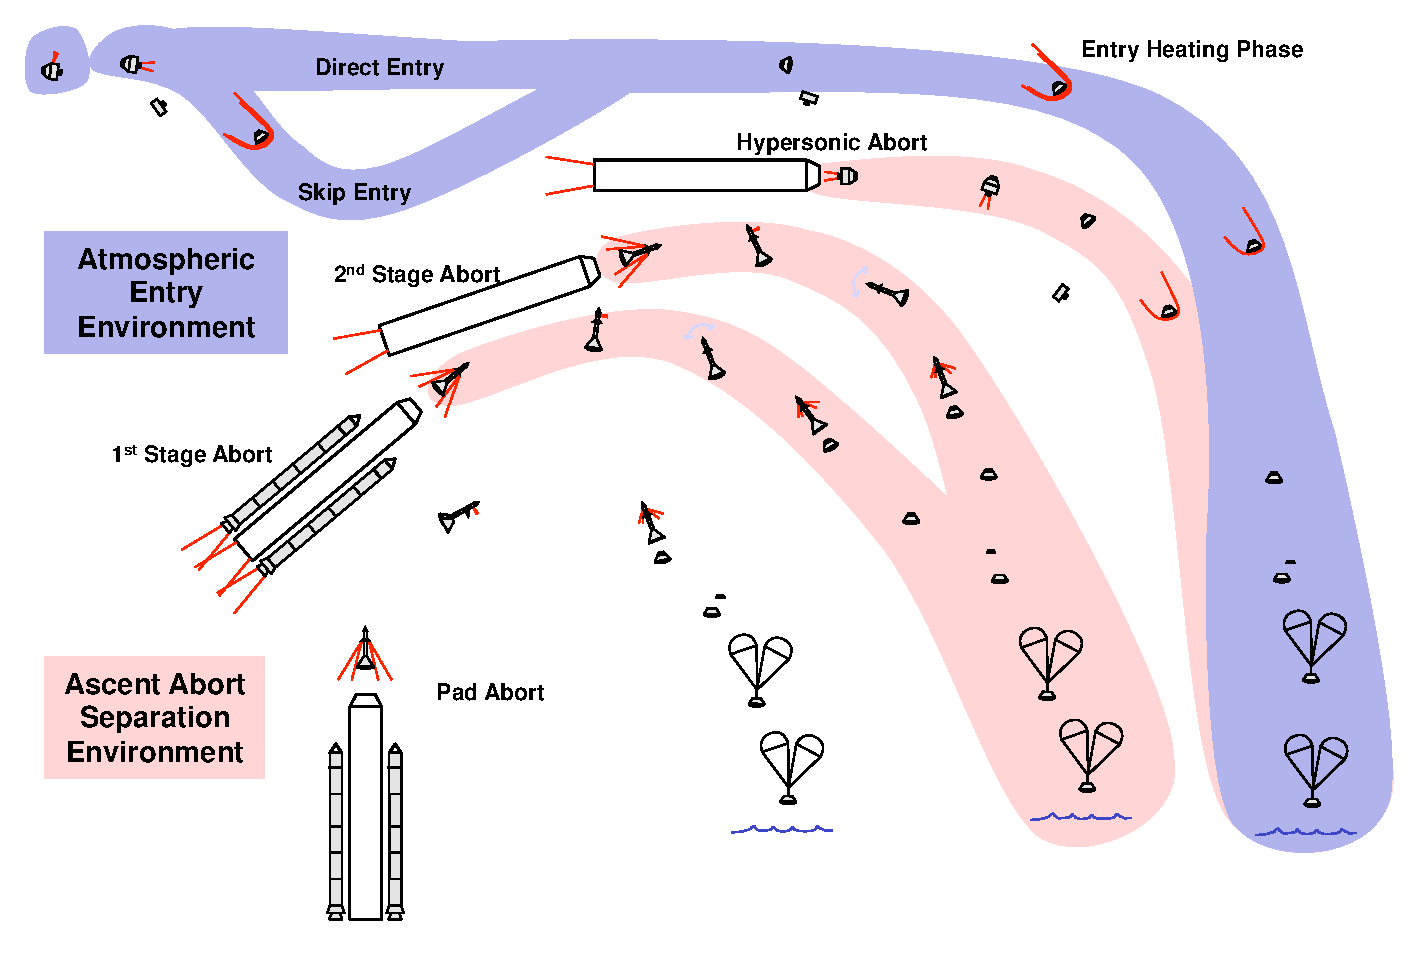
\includegraphics[width=0.85\textwidth]{ResponsibleFlightRegimes}
\\
\vspace{1em}
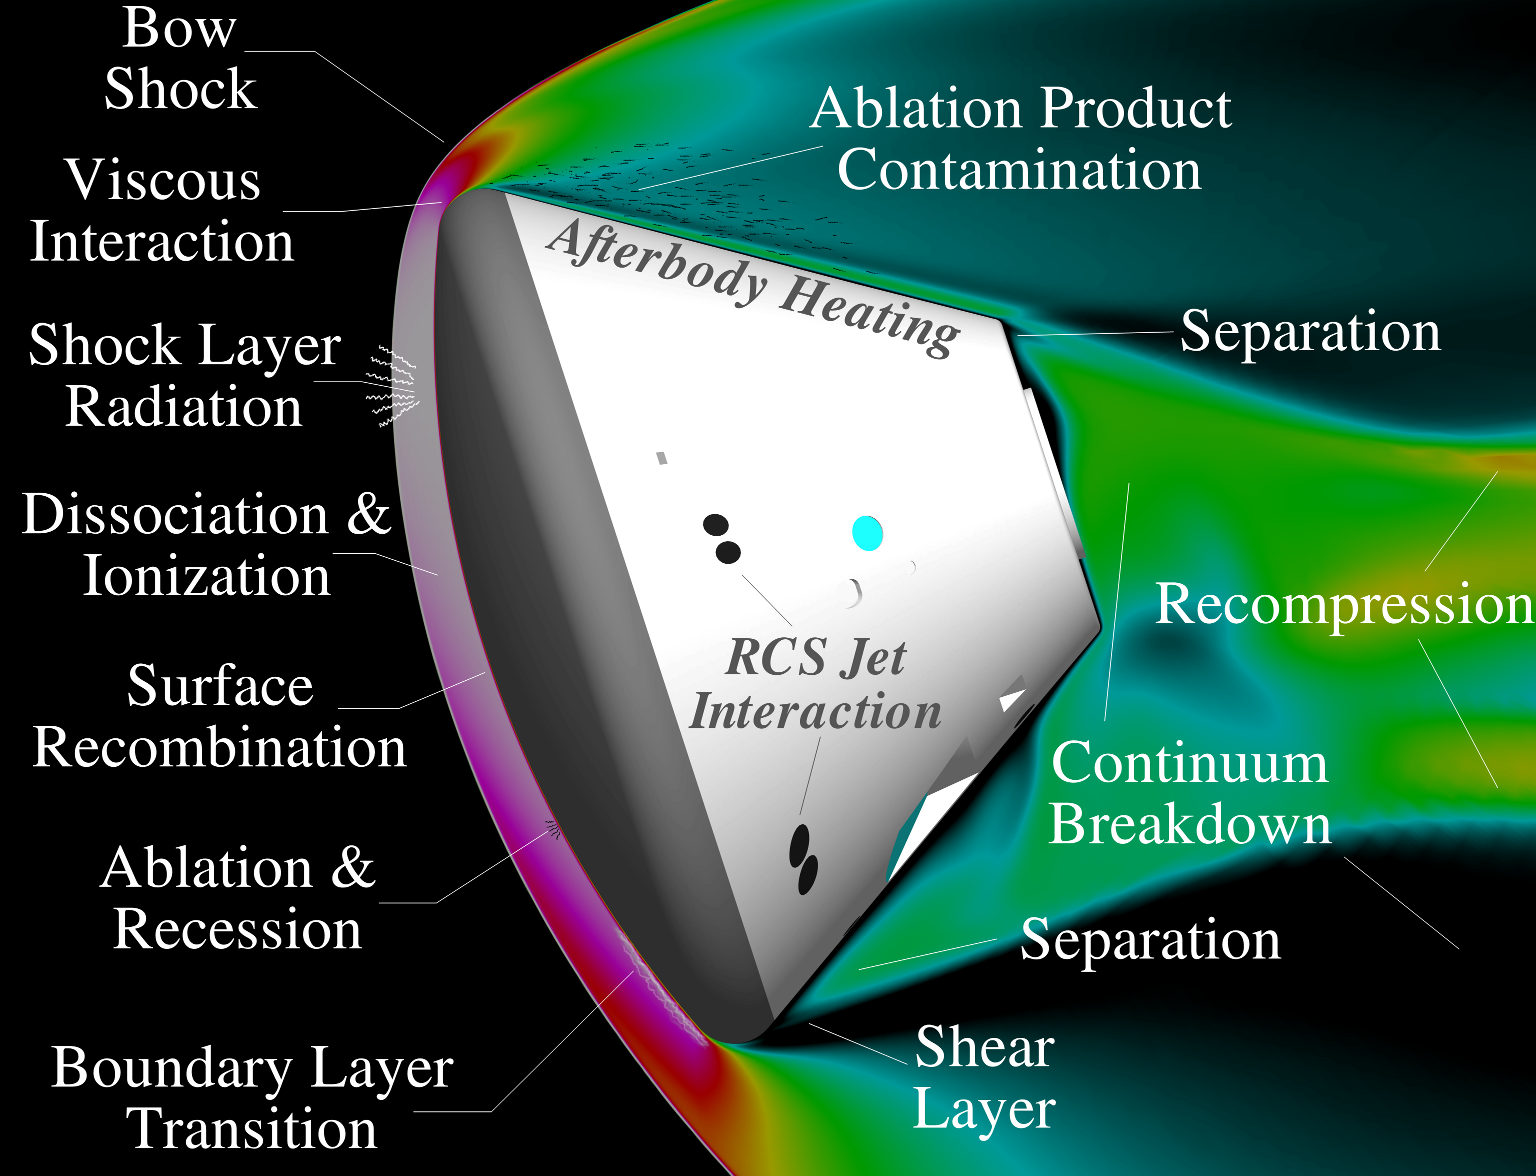
\includegraphics[width=0.48\textwidth]{Capsule_image_updated}
\hfill
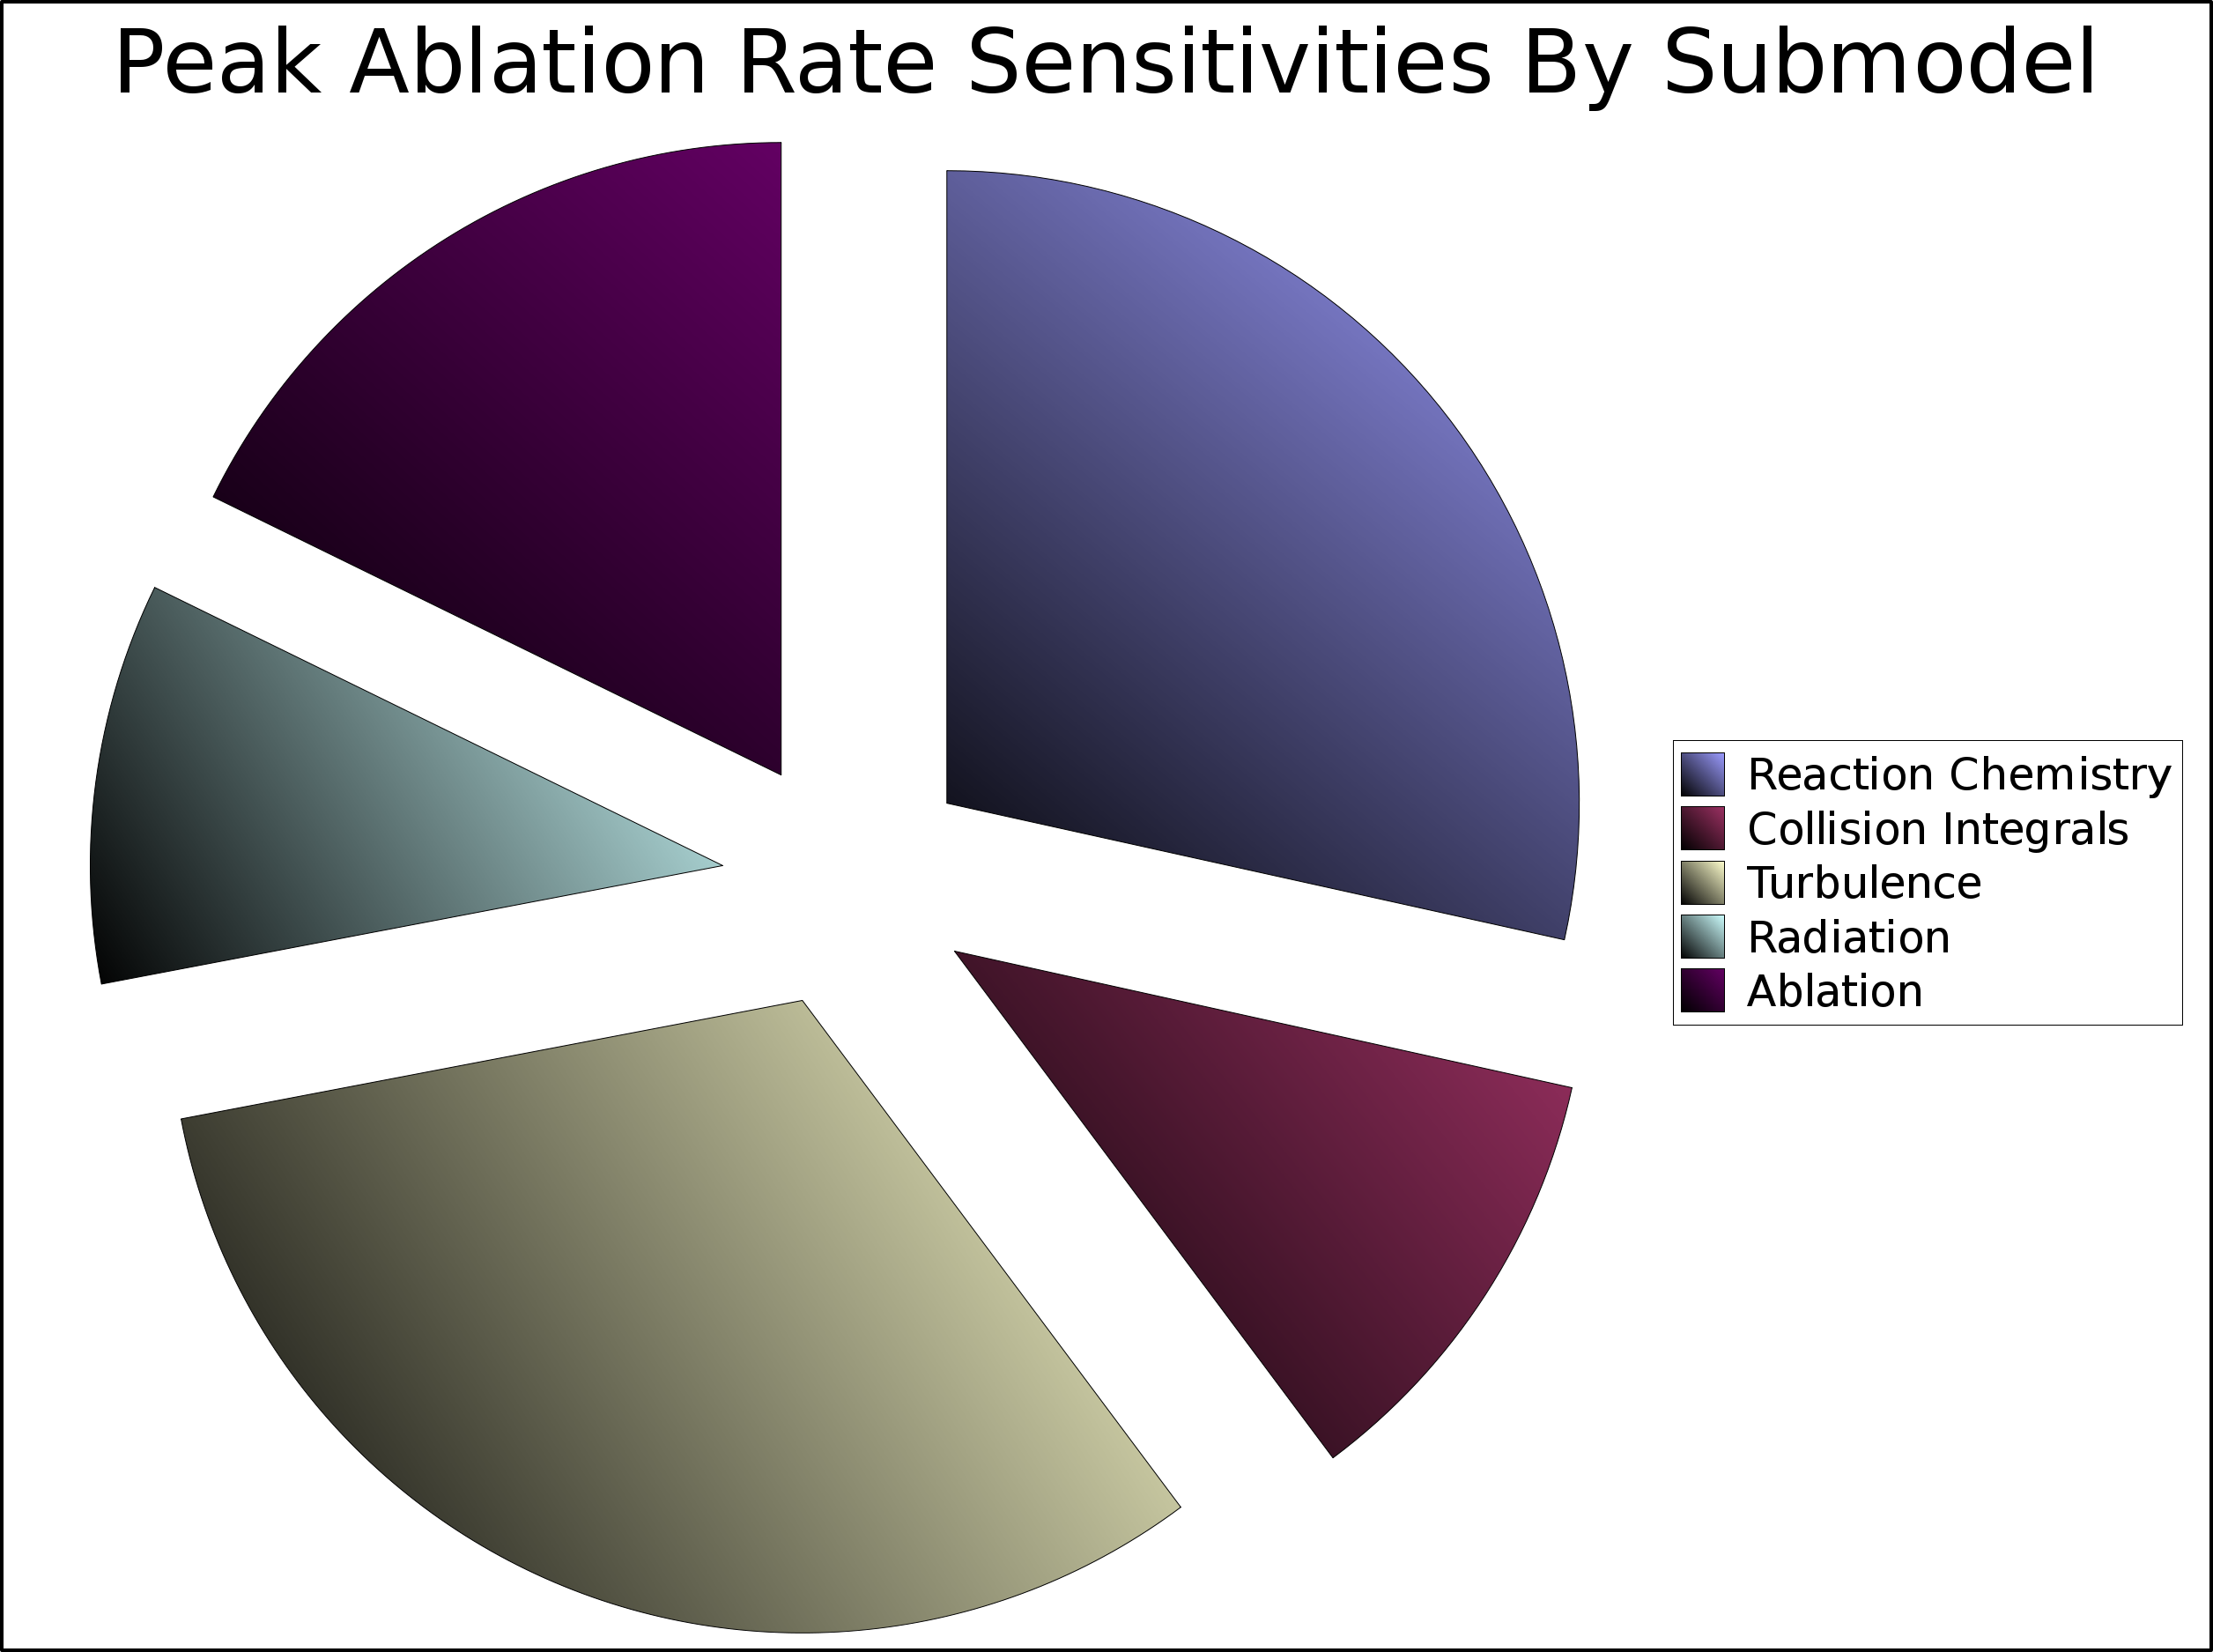
\includegraphics[width=0.495\textwidth]{sensitivity_by_submodel}
\\
\caption[Physics relevant to atmospheric reentry]{%
  The Entry Heating Phase during atmospheric reentry is a complex multiphysics
  problem with uncertainties in system response predictions arising from many
  causes.  In particular, aerothermodynamic heating and any associated ablative
  thermal protection system response predictions are highly sensitive to
  turbulence model parameters.  Top and lower-left images courtesy of NASA\@.
  Lower right image reproduced
  from \citet{Stogner2011Uncertainty}.\label{fig:turbsensitivity}
}
\end{figure}

As part of The University of Texas at Austin's Center for Predictive Engineering
and Computational Sciences'\footnote{\url{http://pecos.ices.utexas.edu/}}
larger investigation into verification, validation, and uncertainty
quantification, \citet{Bauman2011Loose} and \citet{Stogner2011Uncertainty}
performed coupled multiphysics simulations of the blunt-bodied Orion
Multi-Purpose Crew Vehicle (MPCV), then called the Crew Exploration Vehicle
(CEV), undergoing peak heating during return from the International Space
Station.  The upper portion of \autoref{fig:turbsensitivity} shows this
entry heating phase amongst the many other flight regimes in which the
MPCV must operate while the lower left portion depicts the multi-physics
nature of the reentry environment.  The lower right portion of \autoref{fig:turbsensitivity}
reproduces the finding by \citeauthor{Bauman2011Loose} and \citeauthor{Stogner2011Uncertainty} that the
surface heat flux and associated thermal protection system ablation rate showed
more sensitivity to the uncertainties from turbulence models than to any other physics
model they employed.


%%%%%%%%%%%%%%%%%%%%%%%%%%%%%%%%%%%%%%%%%%%%%%%%%%%%%%%%%%%%%%%%%%%%%%%%%%%%%%
\section[Data Requirements for Bayesian Calibration of Turbulence Models]
        {Data Requirements for Bayesian\\Calibration of Turbulence Models}
\label{sec:datareq}

Turbulence modeling is a rich discipline built on theoretical results derived
from first principles, physical intuition obtained from precise measurements,
and, by necessity, judicious curve fitting~\citep{Durbin2011Statistical,
Pope2000Turbulent, Chassaing2010Variable, Wilcox2006Turbulence}.  All
practically useful turbulence models contain imperfectly known free parameters
which must be calibrated via some statistical inference procedure.  For example,
least squares approaches can be used to determine parameters by minimizing the
discrepancy between model predictions and some relevant reference observations,
also known as calibration data.

Recently, Bayesian techniques for turbulence model calibration have been
introduced by \citet{RESS-2010} and expounded upon by \citeauthor{ETC13-2011}
\citep{ETC13-2011, Oliver2012Accounting}.  Following Bayesian philosophy, the
turbulence model parameters,~$\theta$, are assigned a joint prior probability
density function (PDF) characterizing prior knowledge about the
parameters' uncertain, ``true'' values.  During calibration, this prior PDF,
$p_\text{prior}\!\left(\theta\right)$, is merged with a likelihood distribution
depending on new data,~$d$, to obtain a posterior PDF,
$p_\text{post}\left(\theta{}|d\right)$, via Bayes' theorem:
\begin{align}
  p_\text{post}\!\left(\theta|d\right)
  &\propto
  L\!\left(d|\theta\right)
  p_\text{prior}\!\left(\theta\right).
\end{align}
The likelihood function, $L\!\left(d|\theta\right)$, gauges the probability
that the model with parameters~$\theta$ is consistent with the data~$d$.  In
effect, the posterior PDF captures the updated state of model parameter
knowledge obtained by incorporating the calibration data.

Measurement uncertainty in the calibration data is accounted for in the
likelihood function.  By Bayes' theorem, larger measurement uncertainties cause
the calibration data to less strongly influence the posterior PDF which, in
turn, causes less certain turbulence model predictions.  While smaller
uncertainties are therefore desirable, it is far more important that the
calibration data have accurately quantified uncertainties.  Indeed,
inaccuracies poison the posterior PDF.  For these reasons, we say calibration
data is ``high quality'' if, firstly, it is accompanied by accurately
quantified measurement uncertainties and, secondly, if those uncertainties are
small.

Additionally, ``high quality'' calibration data must satisfy
\citeauthor{Settles1991Hypersonic}'s long-established assessment criteria
listed in \autoref{tbl:datacriteria}.  The preceding discussion motivates and
sharpens their requirements regarding \emph{well-defined error bounds}.  Three
of the other criteria are paraphrased briefly as they will be important in the
sequel:
\begin{itemize}
  \item \emph{Realistic test conditions}.  More application-like but
   comparatively rare data are preferred.  For example, in the context of
   reentry vehicles with ablative heat shields, data collected from experiments
   with non-adiabatic walls are preferred.
  %
  \item \emph{Simplicity}. Experimental geometries must be sufficiently simple
  that they may be modeled without enormous difficulty.
  %
  \item \emph{Well-defined boundary conditions}.  All incoming conditions,
  especially the state and ``fluctuating character'' of the incoming
  boundary layer, must be carefully documented.
%%%
%%\item \emph{Turbulent data}.  In addition to mean-flow measurements, data on
%%fluctuating quantities and their correlations are highly desirable.
\end{itemize}
Comprehensive criterion descriptions
% as well as an assessment of the pre-\citeyear{Settles1993Hypersonic}
% calibration data available for $\Mach \geq 3$ boundary layers experiencing
% pressure gradients
appear in~\citet{Settles1993Hypersonic}.

Assuming a predictive model can be validated in a given context
\citep{Oden2010ComputerI, Oden2010ComputerII, Moser2012Validating}, it is the
scarcity of high-quality calibration data that dominates predictive uncertainty.
Because the present work is intended to reduce the uncertainty of aerothermodynamic heating predictions
on blunt-bodied reentry vehicles, and because these predictions are sensitive to
turbulence model parameters, we seek relevant high-quality turbulence
model calibration data.

\begin{table}
\centering
\caption[Data assessment criteria due to \citeauthor{Settles1991Hypersonic}]{%
  While ``\dots{}looking for those few experimental studies of unimpeachable
  quality\dots'' in the super- and hypersonics literature,
  \citet{Settles1994Hypersonic, Settles1991Hypersonic, Settles1993Hypersonic,
  Settles1994Supersonic} set forth these criteria for assessing the utility of
  data sets to the testing and validation of turbulence
  models.\label{tbl:datacriteria}
}
\begin{minipage}[t]{0.97\textwidth}
\hrule
\vspace{0.5\baselineskip}
\begin{minipage}[t]{0.495\textwidth}
  \begin{center}
    Necessary criteria
  \end{center}
  \begin{enumerate}
    \item Baseline  applicability
    \item Simplicity \label{itm:criterion_simplicity}
    \item Specific applicability
    \item Well-defined {boundary conditions} \label{itm:criterion_bcs}
    \item Well-defined error bounds \label{itm:criterion_bounds}
    \item Consistency
    \item Adequate documentation
    \item Adequate spatial resolution
  \end{enumerate}
\end{minipage}
\hfill
\begin{minipage}[t]{0.495\textwidth}
  \begin{center}
    Desirable criteria
  \end{center}
  \begin{enumerate}
    \item Turbulent data \label{itm:criterion_turbulentdata}
    \item Realistic test conditions \label{itm:criterion_realistic}
    \item Non-intrusive instrumentation
    \item Redundant measurements
    \item Flow structure and physics
  \end{enumerate}
\end{minipage}
\vspace{0.5\baselineskip}
\hrule
\end{minipage}
\end{table}


%%%%%%%%%%%%%%%%%%%%%%%%%%%%%%%%%%%%%%%%%%%%%%%%%%%%%%%%%%%%%%%%%%%%%%%%%%%%%%
\section[High-Quality Calibration Data from the Experimental Literature]
        {High-Quality Calibration Data\\from the Experimental Literature}

We seek high-quality experimental data, as defined in \autoref{sec:datareq}, for
supersonic turbulent boundary layers experiencing favorable pressure gradients
that are attached to cold walls possessing either flat or convex geometries.
%
Following earlier data compilations by
\citet{Fernholz1977Critical,Fernholz1980Critical} and \citet{Fernholz1981Further},
\citet{Settles1993Hypersonic} surveyed the 1962--1993 literature to find
experimental data from $\Mach \geq{} 3$ attached turbulent boundary layer flows
in nonzero pressure gradients.  Of the entire corpus then-indexed by the AIAA Aerospace
Database, only nine experimental data sets satisfied their necessary criteria
listed in \autoref{tbl:datacriteria}.  Of those nine, only the work of
\citet{Lewis1972Experiment} included a favorable pressure gradient.  That study
used adiabatic wall conditions,\footnote{Subsequent favorable pressure gradient
experiments by the same authors employed
constant-temperature, cold walls~\citep{Gran1974Effect}.  Though extant, this data was not assessed
by~\citet{Settles1993Hypersonic}} only implicitly reported its error
bounds~\citep[][p.  7201-A-1]{Fernholz1977Critical}, and provided no fluctuating
quantity measurements.  \citeauthor{Settles1993Hypersonic} concluded that both
additional nonintrusive fluctuating flow field measurements and data from
pressure gradient flows having prescribed wall temperatures would be valuable.

Since 1993, experimentalists have generated extensive, nonintrusive
fluctuating data from flows with a variety of pressure gradient
conditions~\citep[e.g.][]{Bowersox1996Combined, Bowersox1996Turbulence,
Arnette1998Effects, Garg1998Measurements, Luker1998Experimental, Latin2000Flow,
Luker2000Influence, Ganapathisubramani2006Largescale, Ekoto2007Planar,
Ekoto2008Supersonic, Ekoto2009Response}.  Explicitly stated, well-characterized
error bounds commonly accompany these more recent measurements.  However,
adiabatic wall conditions continue to overwhelmingly dominate the literature and
experimental data from constant-temperature, cold wall flows remains
comparatively quite rare.  That is, \citeauthor{Settles1993Hypersonic}'s
\emph{realistic test conditions} criterion, discussed in
\autoref{sec:datareq}, remains largely unfulfilled in the current
literature.  Regardless of the wall conditions, obtaining near-wall data also
remains a challenge and limits the utility of experimental measurements for
compressible turbulence model development.

In generally accepted frameworks for predictive
simulation,
high-quality data is unequivocally required for model
validation~\citep{AIAA_Guide_1998, ASME_VV10_2006, ASME_VV20_2009}.\footnote{%
    As defined by \citet{Moser2012Validating},
    ``\ldots validation [determines] whether a mathematical model is a
    sufficient representation of reality \ldots\, for predicting specified
    [quantities of interest] to inform a specific
    decision.''
}  The currently available experimental data sets pertinent to the
scenario of interest are, at best, sufficient for turbulence model
validation~\citep{Roy2006Review}.  Calibration is fundamentally different from
validation in that the data consumed need not be drawn from the system of
interest or some approximate facsimile thereof --- anything
traceable that a practitioner deems informative to a particular model may be
used, provided that the consequential model can be validated.
%%%
%%%In these frameworks, data may be consumed by either procedure but not by
%%%both.\todo{Bob says ``not both''.  Understand, revise.  Drop cuteness.}
%%%As both procedures fight for food from the experimental table but only
%%%calibration can go elsewhere to eat, this work espouses the view that
%%%the scarce, real-world experimental data available should be reserved
%%%for validation alone.
%%%
To make the strongest possible statement, within the above frameworks, about a
model's validity requires assessing it against data not used during calibration.
For these reasons, the present work espouses the view that the scant, high-quality
experimental data available should be reserved for validation alone.


%%%%%%%%%%%%%%%%%%%%%%%%%%%%%%%%%%%%%%%%%%%%%%%%%%%%%%%%%%%%%%%%%%%%%%%%%%%%%%
\section[High-Quality Calibration Data from the Computational Literature]
        {High-Quality Calibration Data\\from the Computational Literature}
\label{sec:highqualitylit}

Direct numerical simulation (DNS) is a high-fidelity computational technique
in which the full spatiotemporal scales of turbulence are resolved numerically.
When performed carefully, DNS accurately captures the dynamics of turbulent
flows permitting unfettered measurement of experimentally inaccessible quantities.
However, because of the need to resolve fine dissipative processes, DNS'
computational expense grows like $\Reynolds^4$ where $\Reynolds$ is an
appropriate Reynolds number.  This explosive
scaling places high Reynolds number flow regimes out of reach of DNS for the foreseeable future.

Fortunately, turbulent boundary layers on blunt-bodied reentry vehicles often
have Reynolds numbers low enough to be accessible by compressible DNS techniques
on current high-performance computing platforms.  Here, the Reynolds number
based on the momentum thickness, $\Reynolds[\theta]{}$, is the pertinent one.
\citet{Bauman2011Loose} found $\Reynolds[\theta]{} \approx 400\text{--}700$ in
their heat shield simulations.  For comparison, \citet{Komminaho2002Reynolds}
reported incompressible DNS results for that same $\Reynolds[\theta]{}$ range in
\citeyear{Komminaho2002Reynolds}.  Though compressible DNS is markedly more
expensive than its incompressible counterpart, computing hardware has improved
by more than an order of magnitude in the interim.

Turbulent boundary layers are more challenging to simulate than
streamwise-homogeneous channel flows because they evolve as they progress
downstream.  If the streamwise direction is treated with aperiodic numerics,
some form of turbulent inflow condition is required.  One common approach is
tripping a laminar profile to cause the flow to transition inside the
computational domain~\citep{Wu1999Simulation}.  Another approach is providing
an approximately realistic turbulent profile via
generation~\citep[e.g.][]{Lund1998Generation}, some auxiliary computation, or
by ``recycling'' rescaled turbulent profiles from elsewhere within the
computation~\citep{Simens2009Highresolution}.  Employing highly efficient,
streamwise-periodic numerics innately forces recycling.  Any chosen technique
brings with it complexity and the danger of introducing unintended
and undesirable
time- and length-scales through the streamwise boundary treatment.

In \citeyear{Schlatter2010Assessment}, \citet{Schlatter2010Assessment} assessed
zero-pressure-gradient, incompressible, low-\Reynolds{} turbulent boundary layer
simulations~\citep{Spalart1988Direct, Komminaho2002Reynolds, Khujadze2007New,
Khujadze2004DNS, Ferrante2005Reynolds, Simens2009Highresolution, Wu2009Direct,
Schlatter2009High, Schlatter2009Turbulent} with the goal of quantifying the
variability of reported results.  \citeauthor{Schlatter2010Assessment} found
``\dots{}surprisingly inconsistent predictions for quantities as basic as the
friction coefficient, shape factor, and fluctuation maxima\dots{}'' despite the
fact that all authors used ``reliable numerical methods with sufficiently high
resolutions.''  They concluded that the discrepancies arose from differences in
inflow Reynolds number and turbulence generation, the amount of settling length
the flow was permitted before it was deemed to have reached its final turbulent
state, and the selection of computational domain dimensions and boundary
conditions.  In short, computational shortcuts anticipated to be benign were
demonstrably not so in subtle ways.

It is reasonable to expect that DNS data sets for compressible boundary layers,
with their additional thermodynamic complexity and greater computational
expense, possess inconsistencies of at least the same severity as their
incompressible counterparts.
%%%
%%% Earlier conclusion that Bob (understandably) commented strongly against
%%%
%%We venture that spatially evolving compressible
%%boundary layer DNS performed at reasonable cost on current computing platforms
%%cannot meet \citeauthor{Settles1993Hypersonic}'s criteria for \emph{simplicity}
%%and \emph{well-defined boundary conditions} discussed in
%%\autoref{sec:datareq}.  Under this assumption, spatially evolving DNS
%%is therefore problematic as a high-quality calibration data source.
%%%
The straightforward consequence is that using spatially evolving compressible
boundary layer DNS as a high-quality calibration data source requires great care
with respect to \citeauthor{Settles1993Hypersonic}'s criteria for
\emph{simplicity} and \emph{well-defined boundary conditions} discussed in
\autoref{sec:datareq}.  Addressing these concerns in the context of a given
data set certainly is possible but is sufficiently difficult\footnote{%
    Confirming that, for example, an inflow-tripping or inflow-rescaling
    procedure has not aphysically perturbed spatially evolving DNS results
    seemingly necessitates performing an auxiliary study checking that reported
    statistics, to reported uncertainties, are insensitive to the
    inflow treatment.  Performing such studies incurs computational expense of
    same order as the original DNS.
}
that finding a less complicated class of calibration data is worthwhile.


%%%%%%%%%%%%%%%%%%%%%%%%%%%%%%%%%%%%%%%%%%%%%%%%%%%%%%%%%%%%%%%%%%%%%%%%%%%%%%
\section[Recent Developments in Homogenization of Turbulent Boundary Layers]
        {Recent Developments in Homogenization\\of Turbulent Boundary Layers}
\label{sec:background_homogenization}

To reduce computational expense and avoid the need for inflow boundary conditions,
\citet{Spalart1988Direct} pioneered the simulation of
spatially homogenized boundary layers.  In his approach, additional
assumptions are introduced to homogenize the boundary layer in the
streamwise direction thus permitting the use of periodic boundary conditions.
Using
\citeyear{Spalart1988Direct} computing hardware,
\citeauthor{Spalart1988Direct} simulated incompressible boundary layers at $\Reynolds[\theta]{}$
up to 1410 which remain among the few widely accepted DNS-derived data sets in the
zero-pressure-gradient turbulent boundary layer
literature~\citep{Honkan1997Vorticity,Wu2009Direct}.
\citet{Guarini1998} extended \citeauthor{Spalart1988Direct}'s work to
spatially homogenized compressible boundary layers, again achieving
considerable expense reduction.  From the perspective of
the current work, homogenization permits better adherence to
\citeauthor{Settles1993Hypersonic}'s criteria for \emph{simplicity} and
\emph{well-defined boundary conditions} because it removes the subtle inflow
boundary condition.

Beyond introducing periodicity, the \citet{Spalart1988Direct} and \citet{Guarini1998} spatial homogenizations add additional ``slow
growth'' forcing terms to the residual of governing equations.  These terms
must be Reynolds-averaged and accounted for during the calibration of the one-
and two-equation turbulence models typically used in super- and hypersonic
applications.  However, taking the Reynolds average of these spatial slow growth forcing terms causes new,
unclosed turbulence correlations to appear which subsequently must be closed
through a modeling ansatz beyond that required to develop the off-the-shelf
turbulence models.  This is undesirable.

Motivated by Rayleigh's problem,
in \citeyear{Topalian2011Slow}
\citet{Topalian2011Slow} sidestepped the appearance of these unclosed terms by
instead homogenizing a temporally evolving boundary layer.  This classical
problem, depicted in \autoref{fig:rayleigh}, concerns the behavior of a fluid
in a semi-infinite domain bounded below by a no-slip wall.  At time $t=0$ the
wall impulsively is started with some constant velocity.  The resulting
boundary layer grows upward as time progresses but is statistically
homogeneous in the streamwise and spanwise directions.

\begin{figure}
\centering
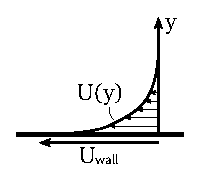
\includegraphics[width=0.30\textwidth]{rayleigh_cartoon}
\caption{Rayleigh's problem. \label{fig:rayleigh}}
\end{figure}

The temporal homogenization approach, to recant from
\citet{Topalian2014Temporal} employing \citeauthor{Spalart1988Direct}-like
notation, begins by manipulating the evolution of a conserved flow quantity
$\phi = \phi[x,y,z,t]$ governed by some nonlinear spatial operator $N$ according
to
\begin{align}
  \pp{\phi}{t} + N[\phi] &= 0.
\end{align}
The quantity $\phi = \bar{\phi} + \phi^\prime$ is decomposed into its mean and
zero-mean fluctuating components, respectively.  Defining $A^\text{RMS}$ to be
proportional to the root-mean-squared fluctuation $\phi^\text{RMS}$,
\begin{align}
 \phi &= \bar{\phi} + A^\text{RMS} \frac{\phi^\prime}{A^\text{RMS}}
       = \bar{\phi} + A^\text{RMS} \phi^\prime_p
\end{align}
where $\phi^\prime_p$ now captures periodic fluctuating behavior.  One
introduces a fast time $t_f = t$ and a slow time $t_s = \epsilon{} t$ where
$\epsilon\ll{}1$ and assumes $\bar{\phi}$ and $A^\text{RMS}$ vary only with
$y$ and $t_s$ while $\phi^\prime_p$ does not vary with $t_s$.  This is
intuitively sensible in Rayleigh's problem as $\bar{\phi}$ and $A^\text{RMS}$
should depend on the slowly evolving boundary layer thickness and the distance
from the wall but not on the field's instantaneous state.  That is,
\begin{align}
 \phi[x,y,z,t] &= \bar{\phi}[y, t_s]
                + A^{\text{RMS}}[y, t_s] \phi^\prime_p[x,y,z,t_f]
  \label{eq:tsg_decomp}
\end{align}
which yields, after some manipulation,
\begin{align}
  \pp{\phi}{t_f} + N[\phi]
  &= -\epsilon \pp{\phi}{t_s}
   = -\epsilon \pp{\bar{\phi}}{t_s}
     -\left( \frac{\epsilon}{\phi^\text{RMS}}
             \pp{\phi^\text{RMS}}{t_s}        \right)\phi^\prime
  \label{eq:tsg_general}.
\end{align}
As alluded to previously, taking the expectation of~\eqref{eq:tsg_general} does
not produce derivatives of mean fast-fluctuating quantities with respect to slow
time.  Consequently, the data produced can be used directly for calibration of
Reynolds-average turbulence models under the additional mild assumption that
modeled quantities, like the turbulent kinetic energy, can also be decomposed
analogously to~\eqref{eq:tsg_decomp}.  The final right hand side
in~\eqref{eq:tsg_general} is the general form of such temporal slow growth
forcing.

Additional work is necessary to completely determine that forcing
and render it in a computable form.  \citet{Topalian2014Temporal} invoked
tensor consistency and self-similarity arguments to permit DNS of a fixed slow
time instant in a zero-pressure-gradient temporal boundary layer.  This
homogenization ultimately adds conserved-quantity forcing terms
\begin{subequations}
\label{eq:temporalhomogenization}
\begin{align}
   &\Ssd_{\rho} = \Ssd_{\rho, t},
   &
   &\Ssd_{\rho u_i} = \rho \Ssd_{u_i,t} + u_i \Ssd_{\rho,t},
   &
   &\Ssd_{\rho E}   = \rho \Ssd_{E,t} + E \Ssd_{\rho,t}
\end{align}
to the fast-time mass, momentum, and total energy equations, respectively.  The
associated specific-quantity forcing terms are
\begin{align}
\Ssd_{\rho,t} &= y \operatorname{gr}_{t_0}\!\left(\Delta\right) \left(
    \frac{\rho}{\bar{\rho}}
    \frac{\partial\bar{\rho}}{\partial\!y}
\right)
\\
\Ssd_{u_i,t} &= y \operatorname{gr}_{t_0}\!\left(\Delta\right) \left(
    \frac{\partial\!\tilde{u}_i}{\partial\!y}
  + \frac{%
      u^{\prime\prime}_i
    }{%
      \sqrt{\widetilde{u^{\prime\prime}_k u^{\prime\prime}_k}}
    }
    \frac{%
      \partial\!\sqrt{\widetilde{u^{\prime\prime}_k u^{\prime\prime}_k}}
    }{%
      \partial\!y
    }
\right)
\\
\Ssd_{E  ,t} &= y \operatorname{gr}_{t_0}\!\left(\Delta\right) \left(
    \frac{\partial\!\tilde{E}  }{\partial\!y}
  + \frac{%
      E^{\prime\prime}
    }{%
      \sqrt{\widetilde{E^{\prime\prime}   E^{\prime\prime}  }}
    }
    \frac{%
      \partial\!\sqrt{\widetilde{E^{\prime\prime}   E^{\prime\prime}  }}
    }{%
      \partial\!y
    }
\right).
\end{align}
\end{subequations}
Here, $y$ is the wall-normal distance and $E$ is the specific total energy.
Tildes denote density-weighted, Favre averages and double primes denote Favre
fluctuations.  To close the model one must supply a temporal growth rate
parameter, $\operatorname{gr}_{t_0}\!\left(\Delta\right)$, which controls the
momentum thickness $\theta$ achieved at stationarity.

Recently, \citeauthor{Topalian2011Slow} augmented their temporal
model~\eqref{eq:temporalhomogenization} with spatial homogenization terms to
model the fast evolution of a homogenized flow defect relative to some
prescribed, spatially developing inviscid base
flow~\cite{Topalian2014Spatiotemporal}.  With an appropriate inviscid base flow
construction, they achieved favorable pressure-gradient-like conditions.  The
construction of this new ``spatiotemporal'' model is technical and has yet to be
published--- a self-contained summary appears in \autoref{sec:imposing_fpg} while
a full derivation is presented in \autoref{sec:slowgrowthmodels}.

The homogenized boundary layers obtained by \citeauthor{Spalart1988Direct},
\citeauthor{Guarini1998}, and \citeauthor{Topalian2014Spatiotemporal} differ
from their physically real, spatially evolving brethren and produce somewhat
different turbulent statistics.  For instance, clearly the former produce
statistically stationary one-dimensional profiles while the latter produces a
two-dimensional profile.  Nevertheless, homogenized boundary layer DNS data is
expected to beneficially inform turbulence model calibration efforts because,
relative to the current state of super- and hypersonic aerodynamic predictions
discussed in \autoref{sec:impact}, it adequately resembles truth data.  In
summary, the present work pursues homogenization because it provides a
reproducible, cost-effective way to produce high-quality calibration data for
turbulence models.

%%%%%%%%%%%%%%%%%%%%%%%%%%%%%%%%%%%%%%%%%%%%%%%%%%%%%%%%%%%%%%%%%%%%%%%%%%%%%%
\section[The Impact of Transition on Aerothermodynamic Heating Predictions]
        {The Impact of Transition on\\Aerothermodynamic Heating Predictions}
\label{sec:transition}

Provided the freestream impinging on a blunt-bodied reentry vehicle has low enough
turbulence, the flow in some neighborhood of the stagnation point will be laminar
because the mean flow velocity must approach zero there.  As favorable pressure
gradients and convex surfaces are well-known to stabilize flows \citep[see,
e.g.,][]{Luker2000Influence,Thomann1968Effect,Arnette1998Effects}, the laminar
region will extend radially outward some distance from the stagnation point.
Discerning, with well-quantified uncertainty, when the flow becomes turbulent is
difficult as laminar-to-turbulent transition processes are highly sensitive
to many environmental details that defy robust
characterization~\citep{Federov2011Transition}.  Indeed, even experimental data
exhibits considerable intra-facility,
observation-to-observation variability as shown in
\autoref{fig:hollis_transition_onset}.  Contributing and compounding in-flight
factors that must be weighed include freestream perturbation levels,
magnification of perturbations as they pass through the bow shock,
chemically reacting ablation products outgassing into the hot flow, and surface
roughness due to ablator fibrosity and possibly spallation.

\begin{figure}
  \centering
  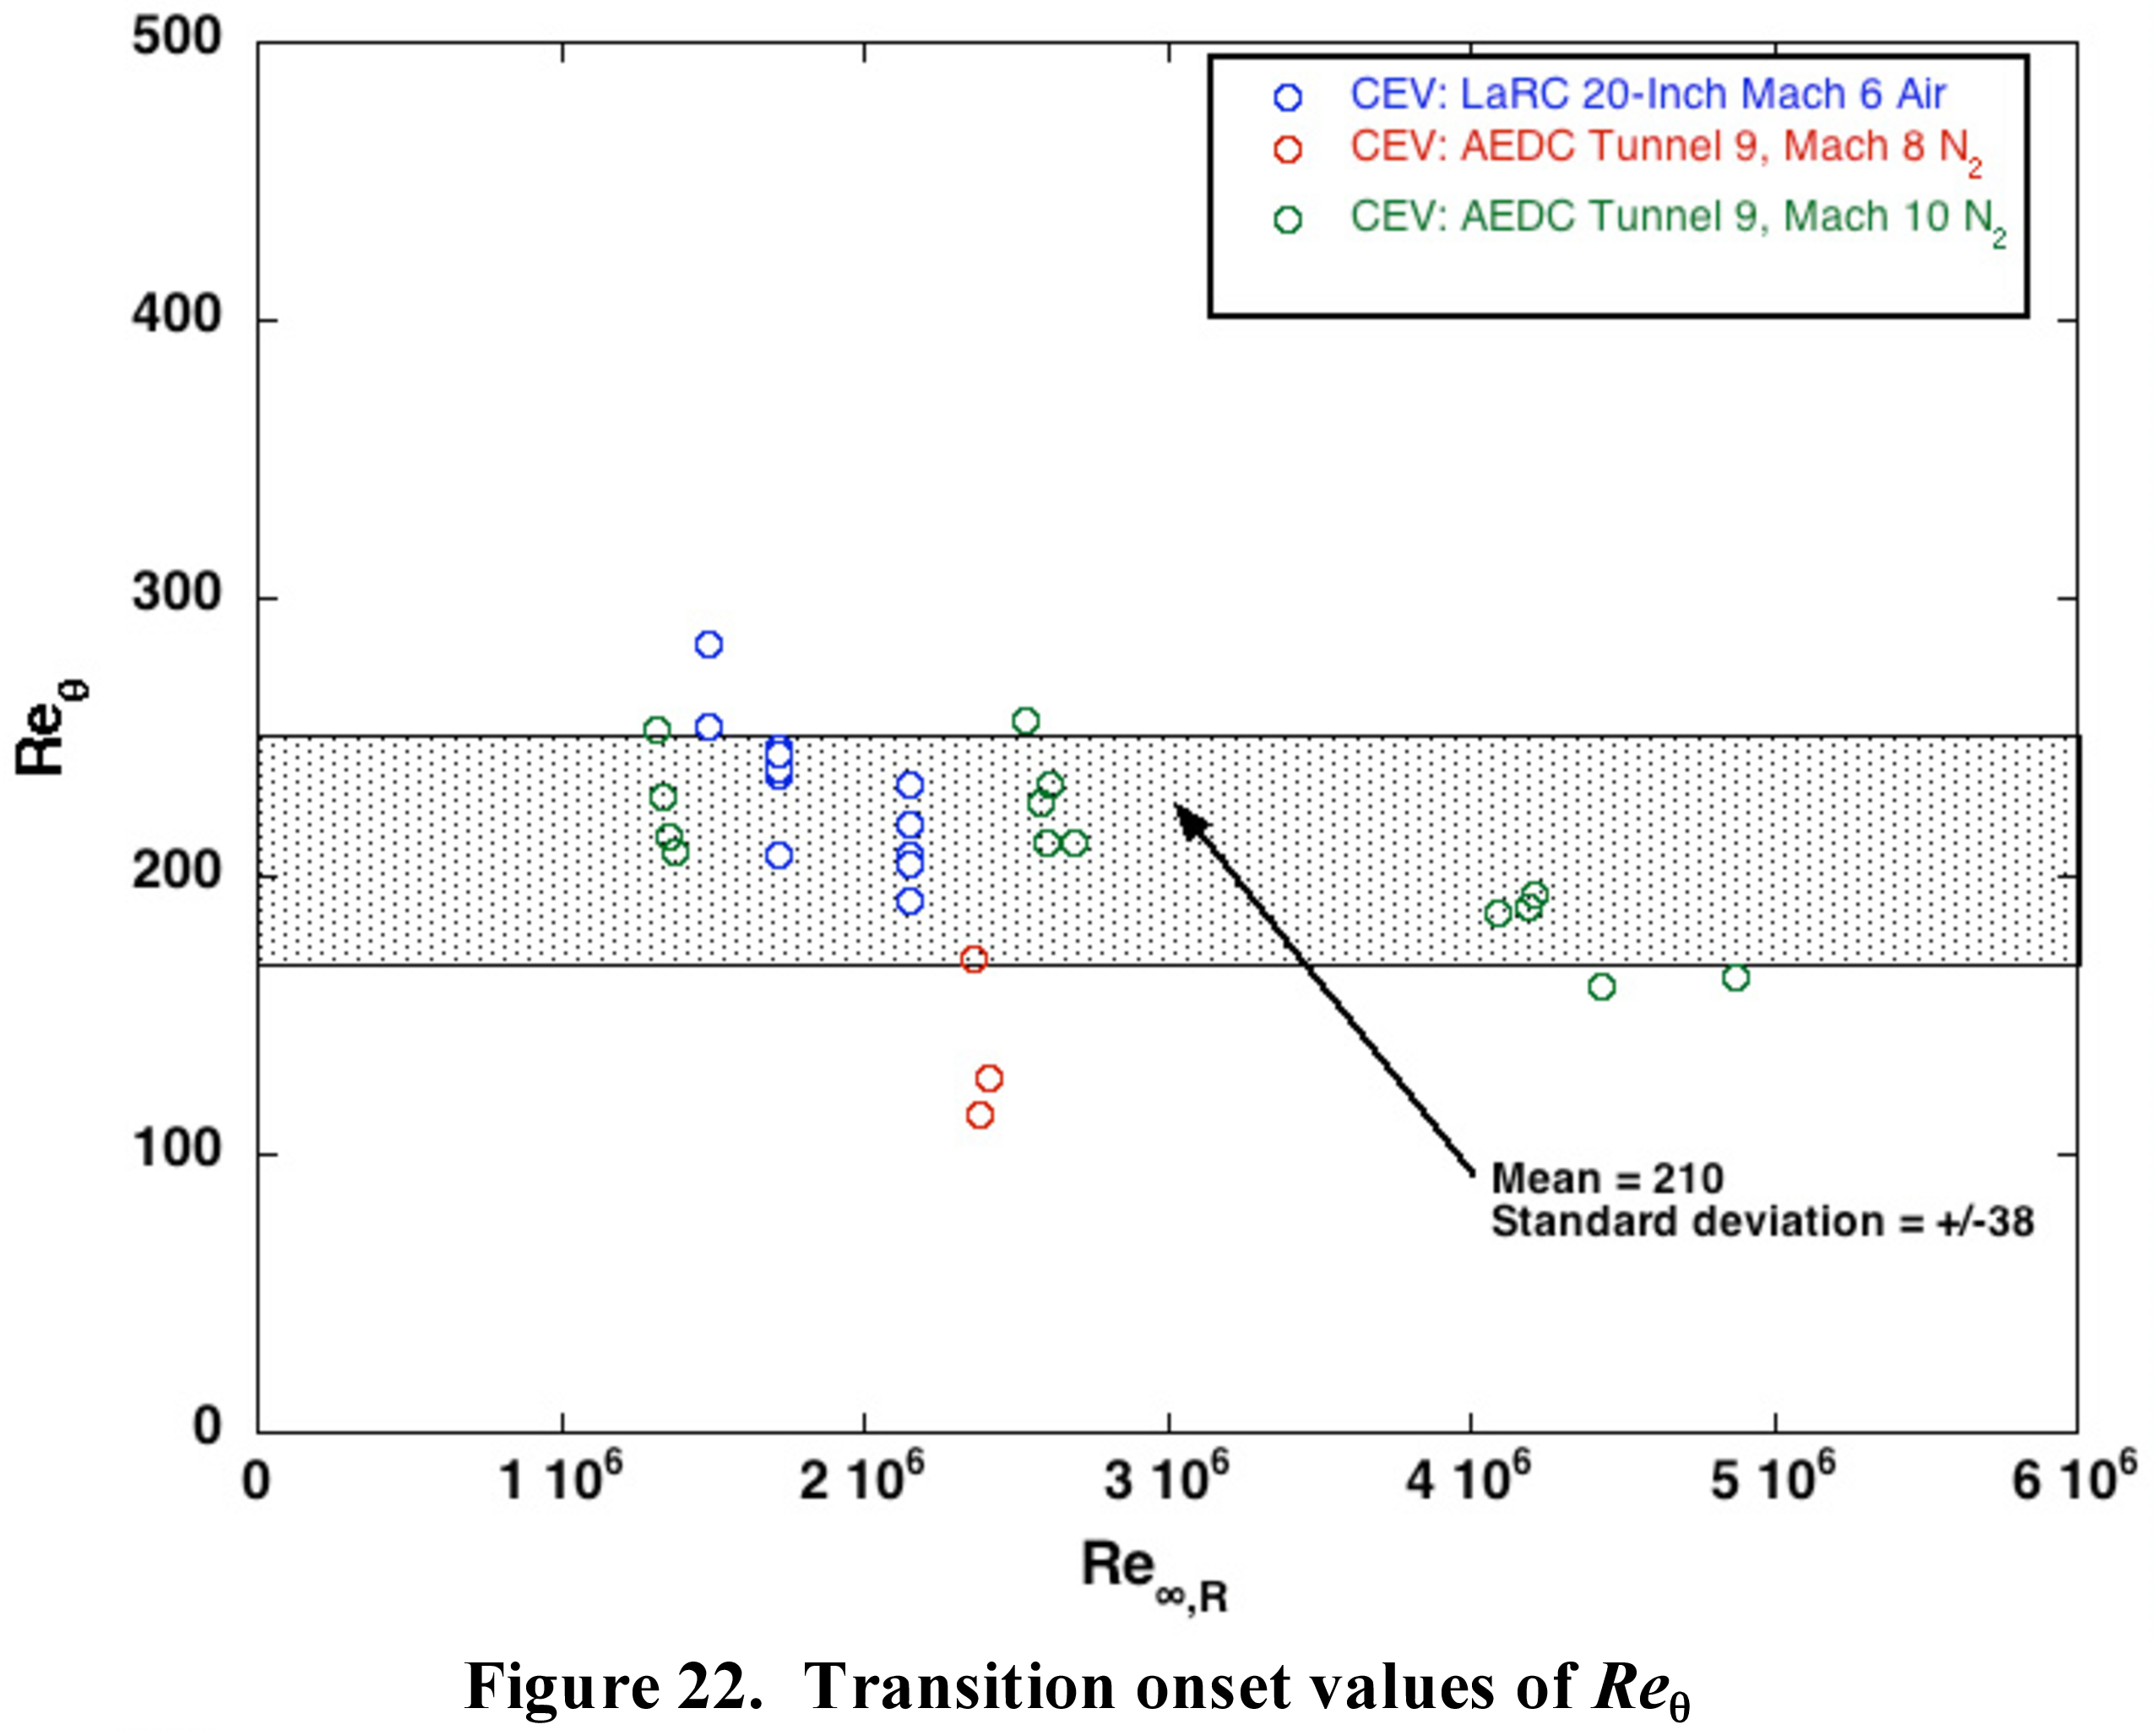
\includegraphics[width=0.72\textwidth]{Hollis2008_Figure22}
  \vfill
  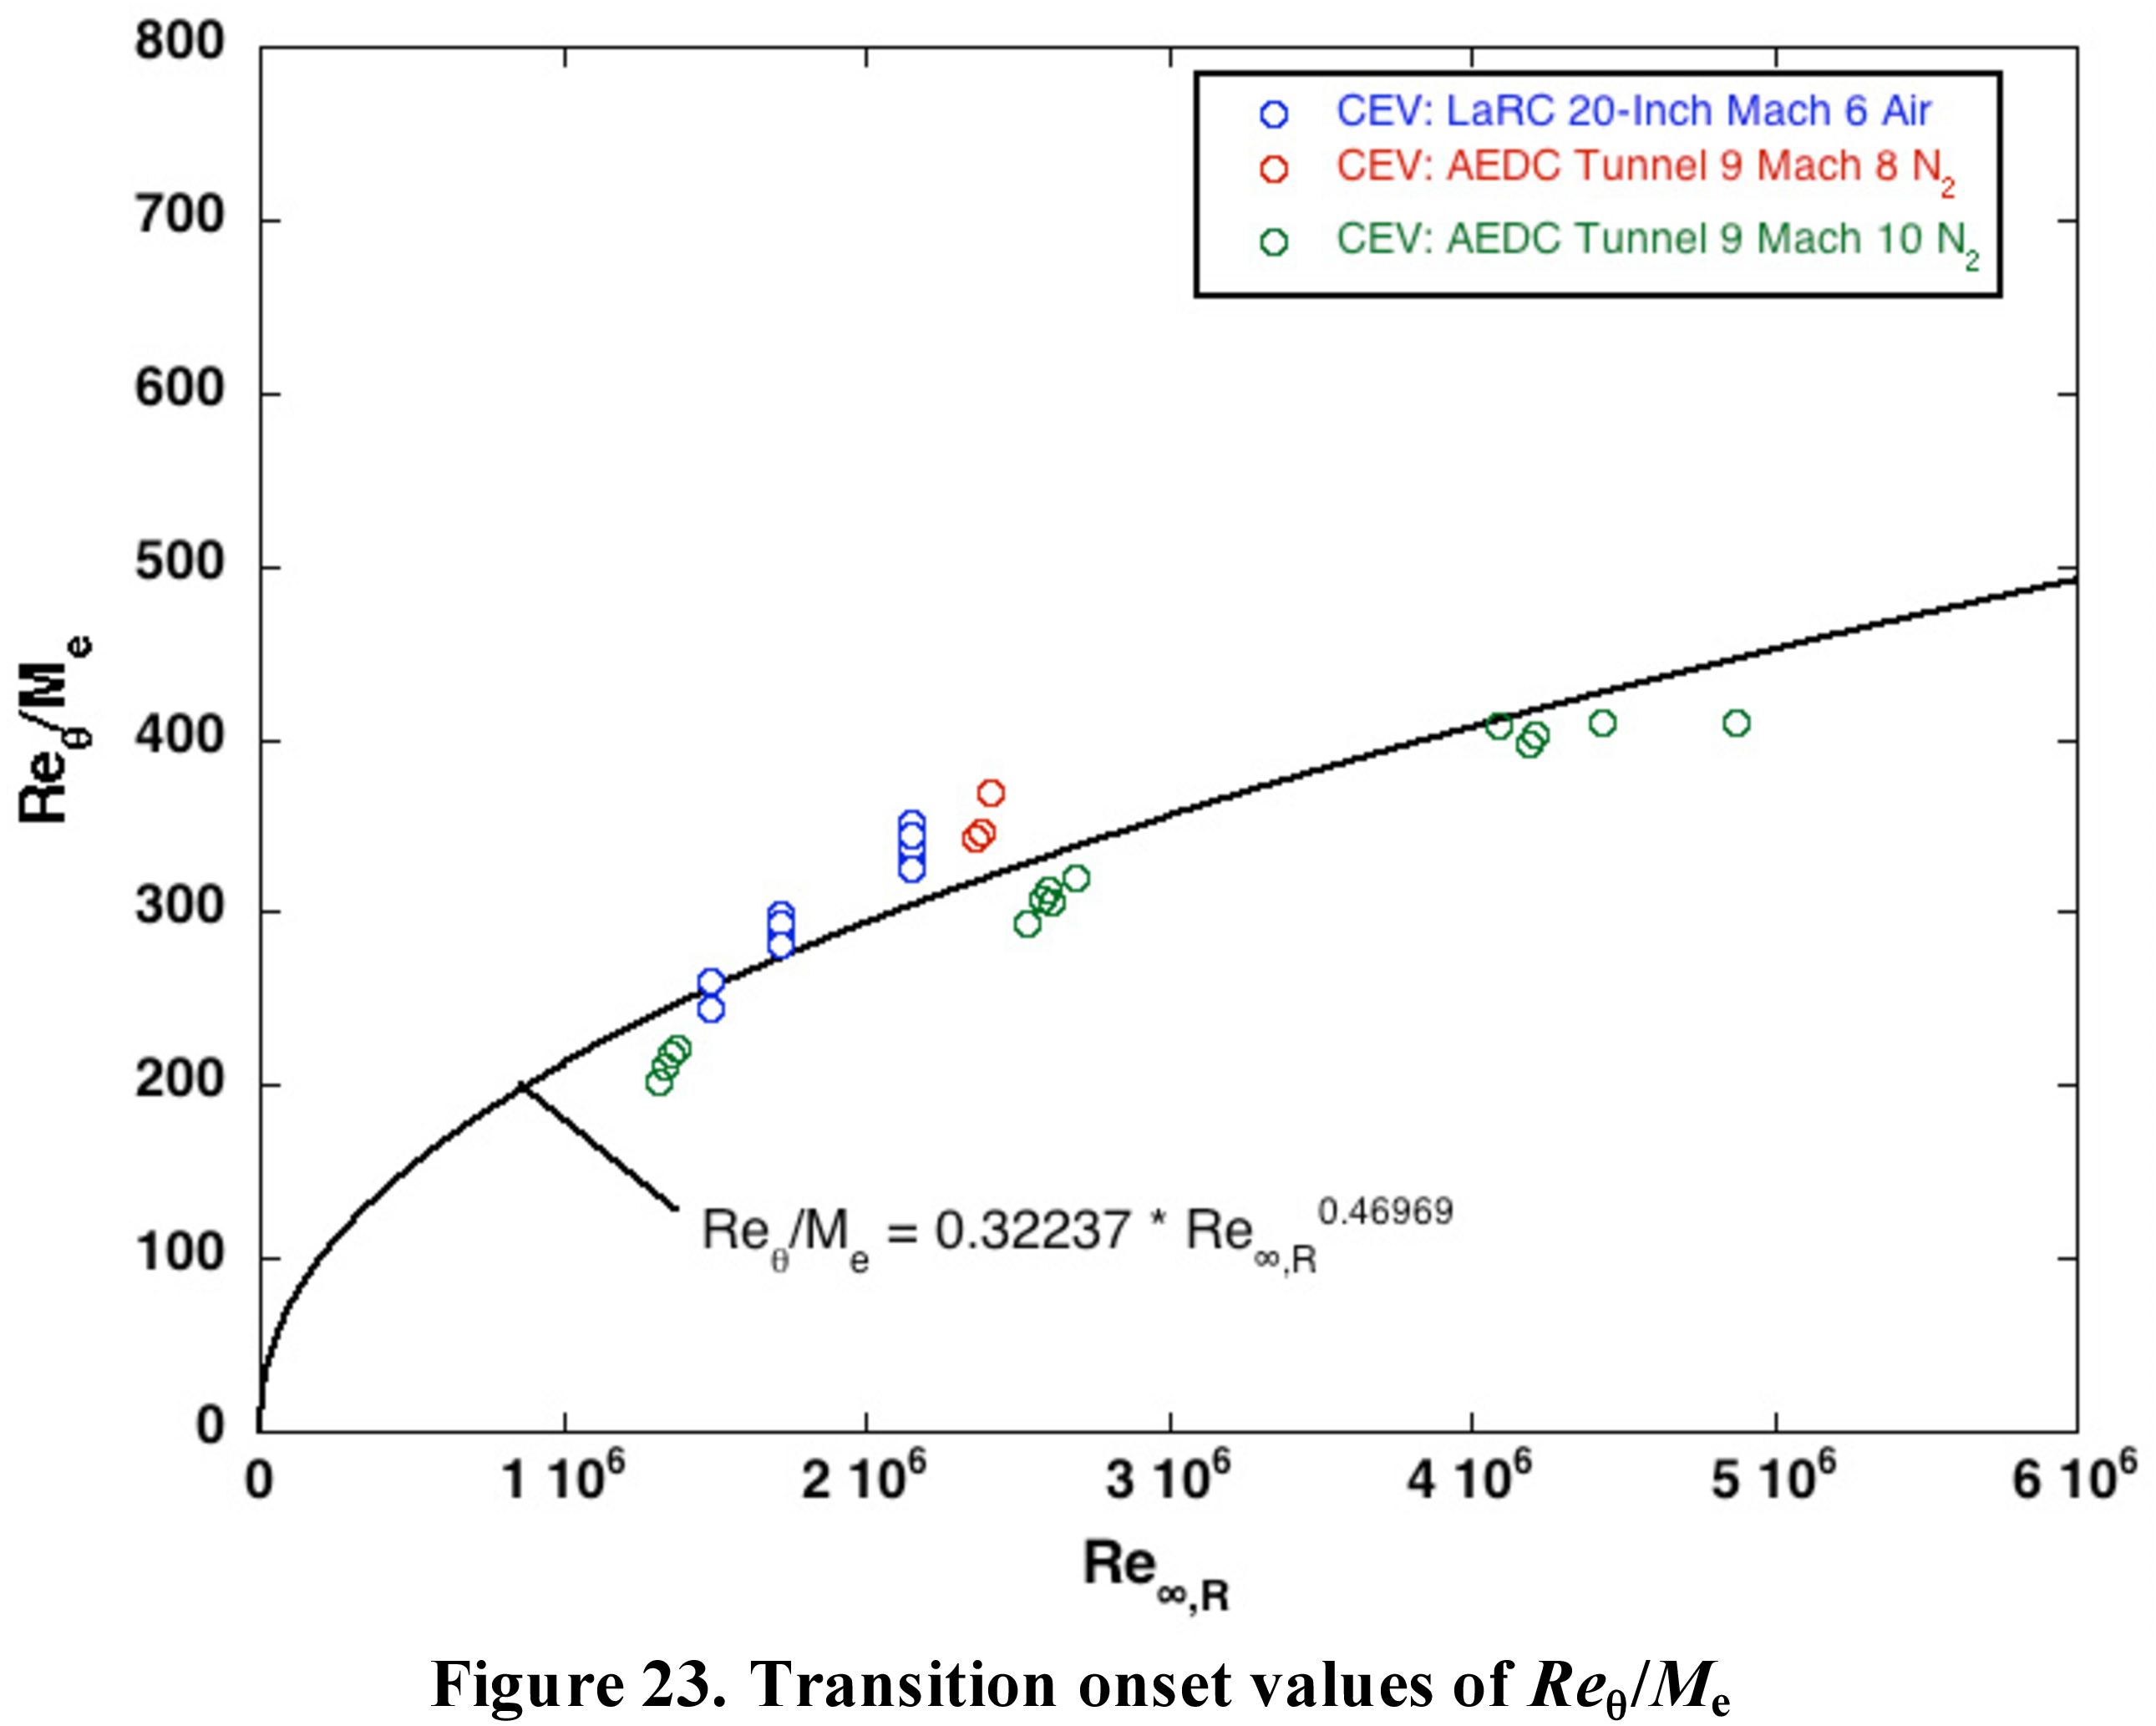
\includegraphics[width=0.72\textwidth]{Hollis2008_Figure23}
  \caption[
      Transition onset values of {$\Reynolds[\theta]{}$} and
      {$\Reynolds[\theta]{} / \Mach[e]{}$} from wind tunnel experiments
      using an Orion MPCV scale model.
  ]{%
      Transition onset values of $\Reynolds[\theta]{}$ (above) and
      $\Reynolds[\theta]{} / \Mach[e]{}$ (below) reproduced from
      \citet{Hollis2008Aeroheating}.  Labels LaRC and AEDC denote the
      NASA Langley Research Center 20-Inch Mach 6 Tunnel and the Arnold
      Engineering Development Center Hypervelocity Wind Tunnel Number 9.
      \label{fig:hollis_transition_onset}
  }
\end{figure}

Engineering estimates of these factors, when inserted into state-of-the-art
transition models, can incur too much uncertainty for engineering use as
\citet{Hollis2008Aeroheating} implied in \citeyear{Hollis2008Aeroheating}:
\begin{quote}
  ``Because of the challenges associated with analysis of all the possible
  transition mechanisms, it is the defined policy of the [Orion MPCV]
  program to make a conservative assumption that the vehicle will
  experience turbulent flow throughout its trajectory.''
\end{quote}
However, using a fully turbulent assumption also impacts aerothermodynamic
heating prediction uncertainty for two reasons.  First, given the high
probability of a laminar region near the stagnation point, the range of feasible
predictions must encompass both globally turbulent and globally laminar
behavior.  The difference between these two behaviors in the context of the
Orion MPCV is depicted in \autoref{fig:normalized_difference}.  Second, again
assuming a laminar region exists, all fully turbulent boundary layer
calculations see incorrect upstream conditions.

\begin{figure}[tb]
  \centering
  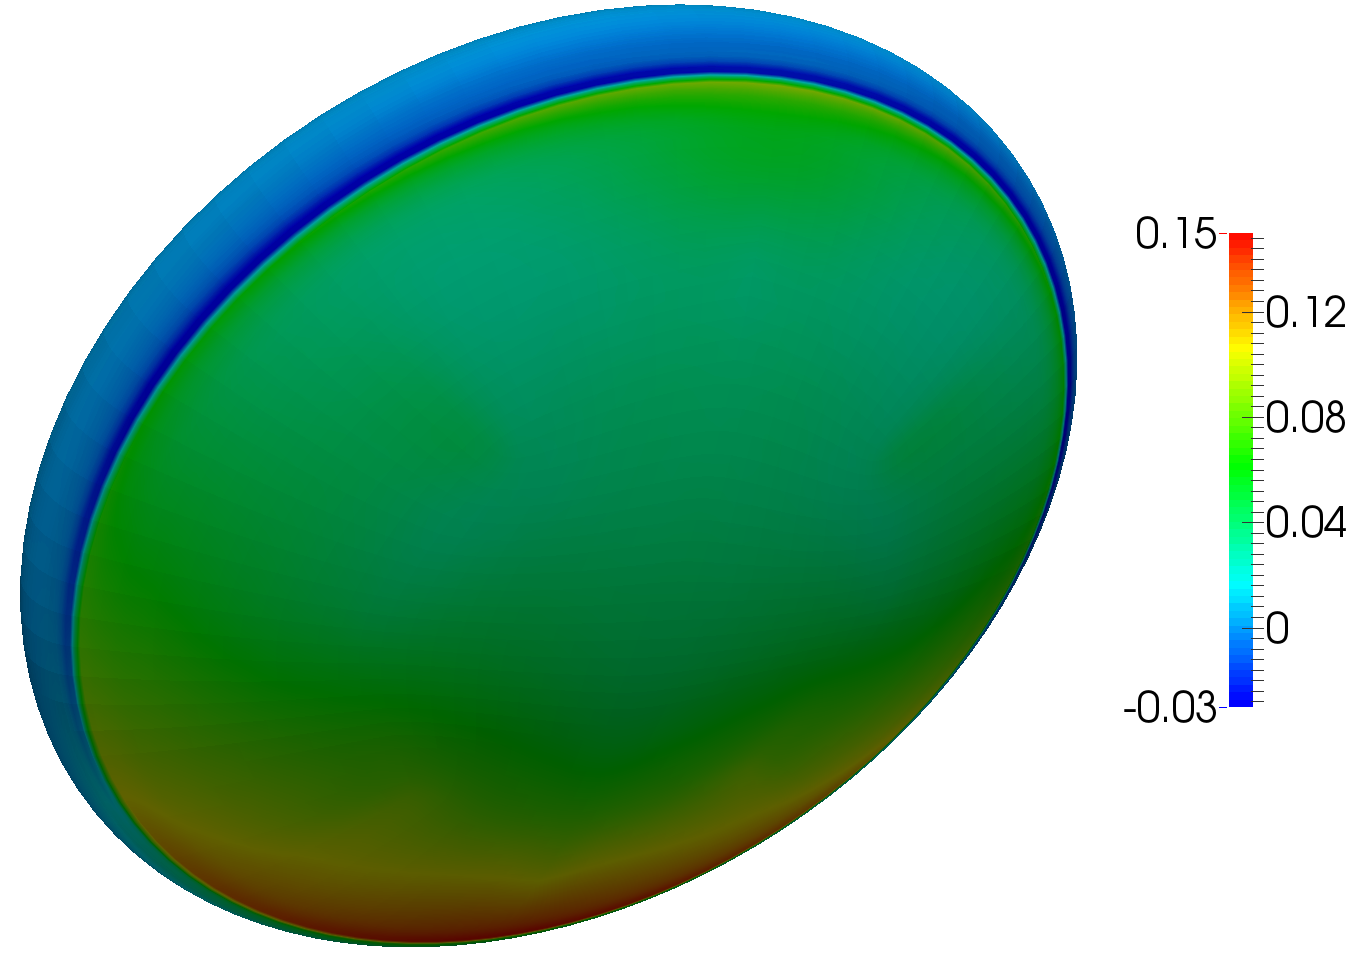
\includegraphics[width=0.85\textwidth]{normalized_difference_white}
  \caption[
    Normalized ablator recession rate difference between fully laminar and fully
    turbulent simulations for Orion MPCV at peak heating conditions from
    International Space Station return trajectory.
  ]{%
    \label{fig:normalized_difference}
    Normalized ablator recession rate difference
    between fully laminar and fully turbulent simulations,
    $\left(\dot{m}_\text{turbulent} - \dot{m}_\text{laminar}\right)
    / \max\left(\dot{m}_\text{turbulent}\right)$, for Orion MPCV at
    peak heating conditions from International Space Station return trajectory.
    Data, which includes aerothermochemistry and ablation, courtesy of P.~T.
    Bauman.
  }
\end{figure}

Aerothermodynamic heating prediction uncertainty would be decreased if one could
reliably use laminar predictions in demonstrably laminar regions and turbulent
predictions everywhere else without incurring the unacceptably large penalty
associated with transition models.  Near-stagnation point laminar prediction
bounds would be tighter and uncertainty in downstream turbulent predictions
would improve as those calculations would subsume more physically correct
upstream information.

One useful bound on the laminar region would be to assume that if local
conditions can at all sustain turbulence, the flow is locally turbulent.  This
bound is reasonable because flight environments contain many perturbation
sources--- any one of which could individually cause transition.  The bound is
conservative because, when used for prediction, turbulent heating is applied as
far upstream as turbulence-enhanced momentum and energy transport to the heat
shield can occur.

Rather than asking where small disturbances induce turbulence, as
transition modeling does, the proposed bound determines where exceedingly
large disturbances are damped, as relaminarization studies
do~\citep{Narasimha1973Relaminarization, Narasimha1979Relaminarization,
Iida1998Relaminarization, Blackwelder1972Largescale,
Schraub1965Study, Ichimiya1998Properties, Talamelli2002Experimental,
Mukund2006Relaminarization, Bourassa2009Experimental}.  Unfortunately,
in their \citeyear{Cal2008Similarity} review of a wealth of experimental
relaminarization data, \citet{Cal2008Similarity} concluded, as
had \citet{Sreenivasan1982Laminarescent} before them, that while
nondimensional parameters~\citep[e.g.][]{Launder1964Laminarization} could
estimate when a flow might revert from turbulent to a ``quasi-laminar''
state, such parameters were not predictive.
%
Given the pragmatic value of finding a predictive bound, it is worthwhile
to investigate analytic results regarding the stability of compressible fluids
to large disturbances with the possibility that these might help rigorously characterize
turbulence-sustaining behavior.

%%%%%%%%%%%%%%%%%%%%%%%%%%%%%%%%%%%%%%%%%%%%%%%%%%%%%%%%%%%%%%%%%%%%%%%%%%%%%%
\section[The Stability of Compressible Flows to Arbitrary Disturbances]
        {The Stability of Compressible Flows\\to Arbitrary Disturbances}
\label{sec:energyperturbationtheory}

The onset of turbulence in a transitional flow is triggered by the nonlinear
growth of small disturbances in the flow field.  The short-time analysis of
the rate of growth of such disturbances is the realm of hydrodynamic linear
stability theory.  In incompressible viscous flows, this process is governed
by the Orr--Sommerfeld equation.  Linear stability theory extends
to compressible, viscous fluids in unbounded domains~\citep{Mack1984Boundary}
and can be used as a transition-prediction mechanism~\citep{Reed1996Linear}.
However, this theory is not useful for studying relaminarization because the
discrepancies between a fully turbulent flow and a steady laminar flow are in
no sense small.

As turbulence can be a self-sustaining process, it is reasonable to assume
turbulent discrepancies from a laminar base flow are somehow pathologically
large.  \citet{Serrin1959Stability}
proved sufficient conditions for the nonlinear stability of an incompressible
viscous fluid in a bounded region to arbitrarily large disturbances using the
energy method.  Suppose one has a base incompressible velocity field
$v$ obeying
\begin{subequations}
\label{eq:serrin_model}
\begin{align}
    \frac{\partial\!v}{\partial\!t} + \nabla\cdot{}v\otimes{}v
&=
  - \frac{1}{\rho} \nabla{} p
  + \nu \Delta{}v
  + f
&
  p, v &\in \Omega
  ,
\\
  v &= v_0
&
  v &\in \partial\!\Omega
\end{align}
\end{subequations}
for some prescribed boundary value $v_0$ where both density $\rho$ and kinematic
viscosity $\nu$ are constant.  The pressure $p$, obtainable from $\Delta{}p = -
\rho \trace \left(\nabla{}v \trans{\nabla{}v}\right)$, instantaneously
maintains $v$ as solenoidal.  Given another admissible $v'$ one may form the
perturbation $u = v' - v$ which evolves locally according to
\begin{subequations}
\begin{align}
  \frac{\partial\!u}{\partial\!t}
&=
  \frac{\partial\!v'}{\partial\!t}
  -
  \frac{\partial\!v}{\partial\!t}
&
  u &\in \Omega
  ,
\\
  u &= 0
&
  u &\in \partial\!\Omega.
\end{align}
\end{subequations}
Taking the scalar product of $u$ with $\partial{}u/\partial{}t$,
employing smoothness, using incompressibility, and simplifying yields the
pointwise evolution of the perturbation energy $E = u^2/2$,
\begin{align}
  \label{eq:reynoldsorr_pointwise}
  \frac{\partial\!E}{\partial\!t}
&=
    \left(
         u \cdot D \cdot u - \nu \nabla u : \nabla u
    \right)
  + \nabla \cdot \left(
      \frac{p-p'}{\rho} u + \nu\nabla{}E - E v'
    \right).
\end{align}
Here, $D = \frac{1}{2}\left(\nabla v + \trans{\nabla v}\right)$ represents the
rate of strain tensor for the base flow.  By the Reynolds transport theorem,
the global perturbation energy may be written
\begin{align}
  \frac{\mathrm{d}}{\mathrm{d}t} \int_\Omega E
&=
  \int_\Omega \frac{\partial\!E}{\partial\!t}
+
  \int_{\partial\!\Omega} E v \cdot \hat{n}.
\end{align}
Using the divergence theorem and that $u = 0 \implies E = 0$ on
$\partial\!\Omega$, gives the Reynolds--Orr energy equation,
\begin{align}
  \frac{\mathrm{d}}{\mathrm{d}t} \int_\Omega E
&=
  \int_\Omega \left( u \cdot D \cdot u - \nu \nabla u : \nabla u \right).
\end{align}
Nondimensionalizing,
\begin{align}
  \label{eq:reynoldsorr}
  \frac{\mathrm{d}}{\mathrm{d}t} \int_\Omega E
&=
  \int_\Omega \left(
        u \cdot D \cdot u
      - \Reynolds^{-1} \nabla u : \nabla u
  \right)
\end{align}
where $\Reynolds = v_0 l_0 / \nu_0$ is the Reynolds number.  The
viscous term always promotes stability but its success in doing so depends on
the relative magnitude of the interaction between the perturbations and the
base flow rate of strain.

\citet{Serrin1959Stability} observed that the base flow $v$ is stable under
arbitrary disturbances as $t\to\infty$ whenever the right hand side of
\eqref{eq:reynoldsorr} is strictly negative for arbitrary, nonvanishing
vectors $u$.  Notice any relevant hysteresis has been implicitly addressed.
Using analytical estimates relying on the boundedness of $\Omega$,
\citeauthor{Serrin1959Stability} characterized critical Reynolds numbers below
which various bounded geometries with steady base flows must be stable to
arbitrary disturbances.  \citet{Joseph1965Stability,Joseph1966Nonlinear}
extended these results to incompressible flows with heat transfer while
\citet{Dudis1971Ekman,Dudis1971Buoyancy} analyzed boundary layers achieving
weaker results due to the unbounded nature of that particular domain.
\citet{Davis1973Reformulation} demonstrated those weaker results could be made
equivalently strong provided
\begin{align}
  \lambda\!\left(t ; D\!\left(t\right), \Reynolds\right)
&= \max \, \frac{%
  \int_\Omega \left(
      u \cdot D \cdot u - \Reynolds^{-1} \nabla u : \nabla u
  \right)
}{%
  \int_\Omega E
}
\label{eq:energy_reform_max}
\end{align}
is well-defined.  The maximum is taken over the space of sufficiently smooth,
divergence-free vector functions satisfying the homogeneous boundary conditions
and behaving appropriately in directions in which the domain is unbounded.  In
particular, the space must permit progressing
from~\eqref{eq:reynoldsorr_pointwise} to~\eqref{eq:reynoldsorr}.
%
%%%Combining~\eqref{eq:reynoldsorr} and~\eqref{eq:energy_reform_max},
%%%\begin{align}
%%%  \frac{\mathrm{d}}{\mathrm{d}t} \int_\Omega E
%%%\leq
%%%  \left. \left(\int_\Omega E\right) \right|_{t=0}
%%%  \lambda\!\left(t\right)
%%%\quad
%%%&\implies
%%%\quad
%%%  \int_\Omega E
%%%\leq
%%%  \left. \left(\int_\Omega E\right) \right|_{t=0}
%%%  \exp \int_0^t \lambda\!\left(s\right)\,\mathrm{d}s
%%%\end{align}
%%%which dominates $\int_\Omega E\to0$ as $t\to\infty$ provided $\int_0^t
%%%\lambda\!\left(s\right)\,\mathrm{d}s \to-\infty$ in the same limit.
%
\citeauthor{Davis1973Reformulation} reformulated the maximization problem
\eqref{eq:energy_reform_max} using the equivalent Euler--Lagrange equations to
numerically obtain critical Reynolds numbers below which oscillatory Stokes
layers must be asymptotically stable.  Estimates for exterior domains
not relying on numerical solutions can be found
in \citet{Galdi1983Local,Maremonti1984Asymptotic}.

In problems where thermodynamic properties vary, the identity analogous to
\eqref{eq:reynoldsorr} additionally must incorporate property perturbation
energies.  For example, \citeauthor{Joseph1966Nonlinear} chose $E = u^2 +
\Prandtl{}\,T^2$ when studying buoyancy problems characterized by a Prandtl
number~\Prandtl{} in which temperature perturbations $T$ were present.  The predictive
quality of the resulting estimates depends strongly on such choices and good
selections are by no means obvious~\citep{Galdi1985Nonlinear}.
\citet{Galdi1990New} set forth an abstract framework providing guidance on
energy identity selection techniques producing promising estimates.

Working within this framework, \citet{Padula2011Asymptotic} cataloged extensive
stability proofs for barotropic and polytropic compressible viscous
fluids.\footnote{%
An exemplary, earlier appearance of the barotropic
results~\citep{Padula2000Stability} is recommended as an introduction.
}
The latter class is therein proved asymptotically stable when bounded by rigid
boundaries provided the initial temperature gradient is sufficiently
small~\citep[theorem~2.4.20]{Padula2011Asymptotic}.
\citeauthor{Padula2011Asymptotic} conjectured that this proof may be extended
to the boundary layer~\citep[page 207]{Padula2011Asymptotic} similarly to how
she obtained boundary layer results for isothermal
fluids~\citep[\textsection\textsection{}2.4.1--2,
\textsection{}4]{Padula2011Asymptotic}.

Any such proof of the asymptotic stability of a compressible viscous boundary
layer to arbitrary disturbances, whether or not it is extended from the work of
\citeauthor{Padula2011Asymptotic}, must simultaneously address several issues.
First, the space chosen must permit exact pointwise perturbation evolution
equations like~\eqref{eq:reynoldsorr_pointwise} to be converted to global
statements like~\eqref{eq:reynoldsorr} despite the unbounded nature of the
domain.  Second, these global evolution statements for perturbation energies
$\rho^2$, $u^2$, $T^2$, etc.\@ must be combined into a single, appropriately
weighted identity.  Third, the evolution of that single identity must either be
bounded using a host of analytical estimates or a
maximization problem resembling~\eqref{eq:energy_reform_max} must be solved
numerically.
Finally, for the proof to be practically useful to those studying
relaminarization, the provably stable region within the parameter space
consisting of $\Reynolds$, $\Prandtl$, etc.\@ must be reasonably sharp relative
to the ``true bounds'' one could hypothetically observe in engineered systems
like the Orion MPCV.
%
Though no currently known asymptotic stability estimate applies to the present
work, energy method concepts and, in particular, interpreting turbulence as a
large, self-sustaining perturbation will be important to the discussion in
\autoref{sec:relam}.

%%%%%%%%%%%%%%%%%%%%%%%%%%%%%%%%%%%%%%%%%%%%%%%%%%%%%%%%%%%%%%%%%%%%%%%%%%%%%%
\section[Bounding Turbulence-Sustaining Regions via Homogenized Simulation]
        {Bounding Turbulence-Sustaining Regions\\via Homogenized Simulation}
\label{sec:detectingrelaminarization}

Absent practical, analytical methods for characterizing turbulence-sustaining
regions at the experimentally inaccessible flight conditions of interest,
simulation is a logical tool to exploit.  Studying the relaminarization of
spatially evolving boundary layers is subject to the issues raised in
\autoref{sec:highqualitylit}.  However, the spatiotemporal homogenization
approach by \citet{Topalian2014Spatiotemporal}, mentioned in
\autoref{sec:background_homogenization}, does permit numerically investigating
this class of flows while avoiding reproducibility problems and excessive
computational cost.  The present work pursues this approach.

A homogenized relaminarization study takes as its input the steady flow field
experienced by the vehicle's thermal protection system during peak heating from
some reentry trajectory.  This ``full system'' of interest should be computed
with the maximum possible fidelity~\citep{Kirk2014Modeling,
Wright1996Dataparallel, Nompelis2005Parallel} in all respects save for assuming
fully laminar conditions.  Fully turbulent, homogenized flow fields are prepared
at local conditions taken from those laminar full system computations.  The
local conditions are said to be unable to sustain turbulence if the field
relaminarizes.  The parameter space of local conditions is searched by
traversing the two-dimensional surface of the full system simulation.  Starting
from just upstream of the heat shield's edge, the relaminarization tests are
repeated at local conditions taken closer and closer to the stagnation point
until the edge of the turbulence-sustaining region is detected.

By using laminar full system conditions as ``upstream'' input, the present
study aims to answer where on a mixed laminar-turbulent heat shield
the local flow conditions can sustain turbulence.  That is, this approach
enjoys independence from the uncertainties associated with turbulence modeling.
%
A different question is, can the entire thermal protection system
surface be turbulent?  That question could be addressed partially by taking as
input the local conditions from assumed-turbulent computations of the full
thermal protection system.  However, such work would carry appreciably greater
uncertainty because the required full system simulations would employ turbulence
models.

Two issues merit immediate attention.  First, the purely temporal forcing terms
from~\eqref{eq:temporalhomogenization} and their spatiotemporal brethren to be
relayed in \autoref{sec:imposing_fpg} are formally ill-defined in the laminar
limit because both $\sqrt{\widetilde{u^{\prime\prime}_k u^{\prime\prime}_k}}$ and
$\sqrt{\widetilde{E^{\prime\prime} E^{\prime\prime}}}$ must eventually vanish there.
However, when subject to relaminarizing conditions, turbulent flows tend
towards a ``quasi-laminar'' state~\citep{Sreenivasan1982Laminarescent} in which
nontrivial streamwise fluctuations persist though turbulent production becomes
nearly zero~\citep{Cal2008Similarity}.  Second, the extent to which
relaminarization processes in a homogenized boundary layer reflect those
in a spatially evolving boundary layer is admittedly unknown.  That said, for
predicting the initial onset of relaminarization, the homogenized treatment is
likely more conservative than the spatially evolving flow because disturbances
cannot exit a homogenized simulation's periodic domain.

The concrete scenario investigated for its turbulence-sustaining region is
taken from Orion MPCV thermal protection system simulations discussed
in the following section.  To keep the calculations tractable, in
the current work aerothermochemistry is neglected and the ablative
conditions are emulated by wall transpiration.  Convex surface curvature,
which has a stabilizing impact~\citep{Bowersox1996Turbulence}, is
also neglected as it cannot be accommodated by the spatiotemporal
homogenization.  The parameter space of local conditions, to be detailed
in \autoref{sec:orionmpcv}, consists of the Reynolds number
based on momentum thickness, the Mach number, the pressure gradient
strength, the wall transpiration rate, and the coldness of the wall
relative to the boundary layer edge.

%%%%%%%%%%%%%%%%%%%%%%%%%%%%%%%%%%%%%%%%%%%%%%%%%%%%%%%%%%%%%%%%%%%%%%%%%%%%%%
\section[Peak Heating Conditions on the Orion Multi-Purpose Crew Vehicle]
        {Peak Heating Conditions on the\\Orion Multi-Purpose Crew Vehicle}
\label{sec:orionmpcv}

%%%EVIL%EVIL%EVIL%%%
\enlargethispage{1.70em}
%%%EVIL%EVIL%EVIL%%%
%
The NASA Orion\footnote{\url{http://www.nasa.gov/orion/}} Multi-Purpose Crew
Vehicle (MPCV) concept was recommended by NASA's Exploration Systems
Architecture Study in 2005 under the earlier Crew Exploration Vehicle (CEV)
moniker~\citep[\textsection{}5]{NASA2005CEVReport}.  Configurations of this
vehicle are intended to transport a crew of four-to-six during International
Space Station, Lunar, and Mars mission scenarios.  Its roughly 5-meter-diameter,
Avcoat-based, ablative heat shield uses sacrificial epoxy novolac resin in a
fiberglass honeycomb matrix to withstand temperatures of roughly 3,600
K~\citep{SpaceCom20130722} while limiting the thermal exposure of the
protected components to only 450
K~\citep[\textsection{}5.3.1.3.7]{NASA2005CEVReport}.
\autoref{fig:cev_scalecomp} provides a sense of scale for this heat shield while
\autoref{fig:cev_symplane} depicts one possible orientation relative to oncoming
flow.  An unmanned, heavily instrumented reentry as part of NASA's
Exploration Flight Test-1 is currently planned to occur during December
2014~\citep{SpaceCom20140317}.

\begin{figure}[p]
  \centering
  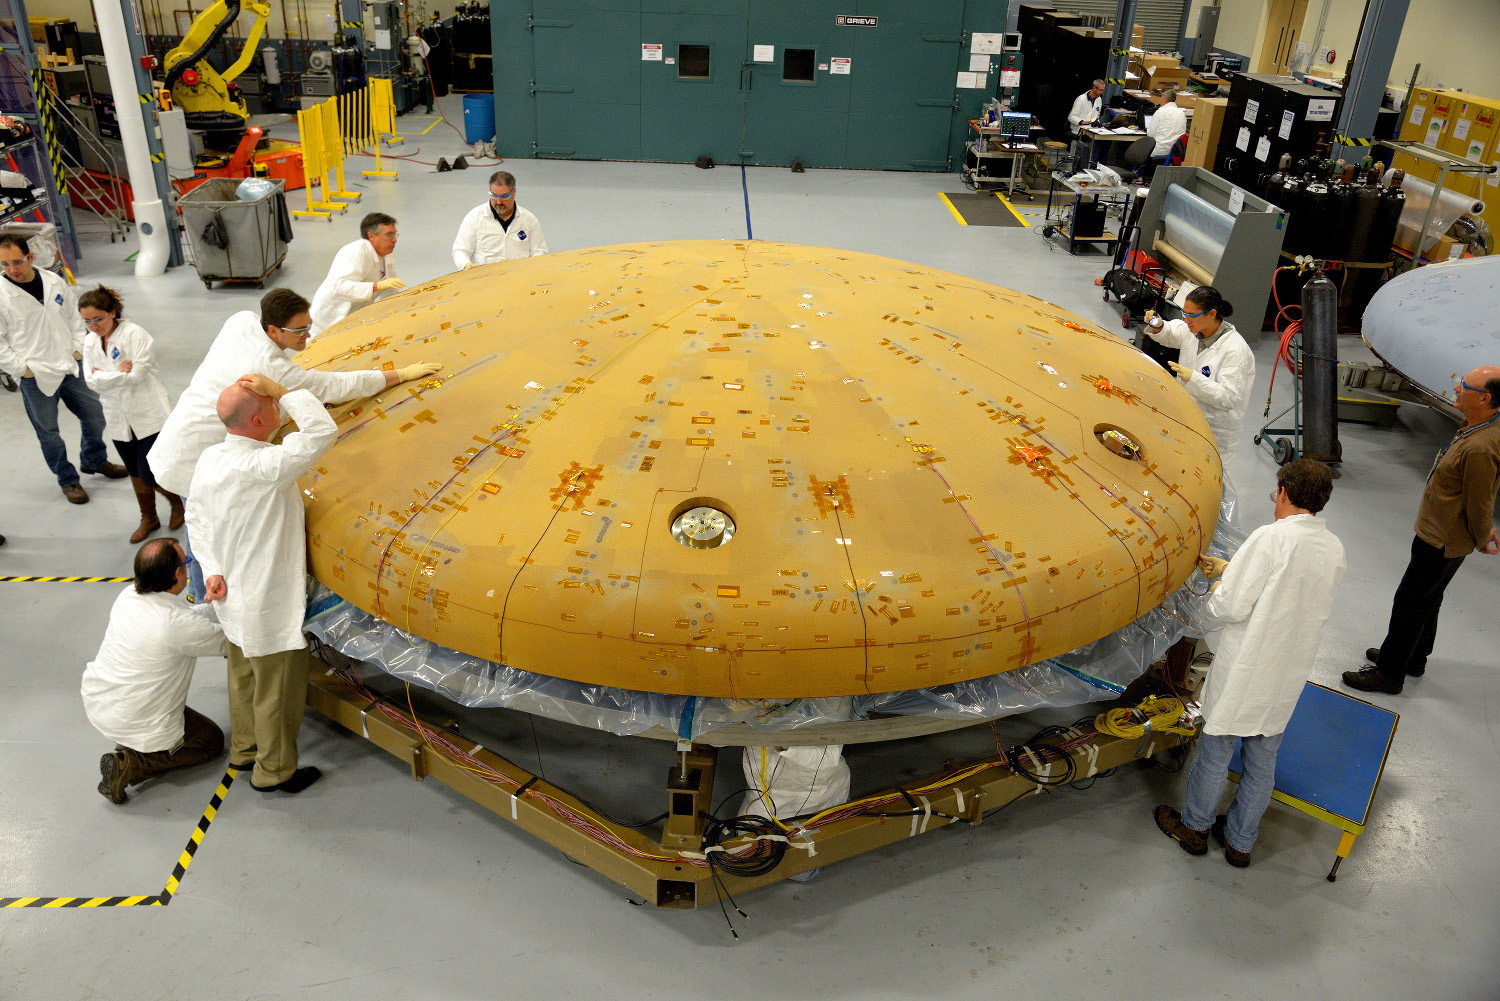
\includegraphics[height=0.35\textheight]{OrionTPSScale_small}
  \caption[
    Scale comparison for the Orion MPCV thermal protection system.
  ]{%
    \label{fig:cev_scalecomp}
    Scale comparison for the Orion MPCV TPS\@.  Image courtesy of NASA.
  }
\end{figure}

\begin{figure}[p]
  \centering
  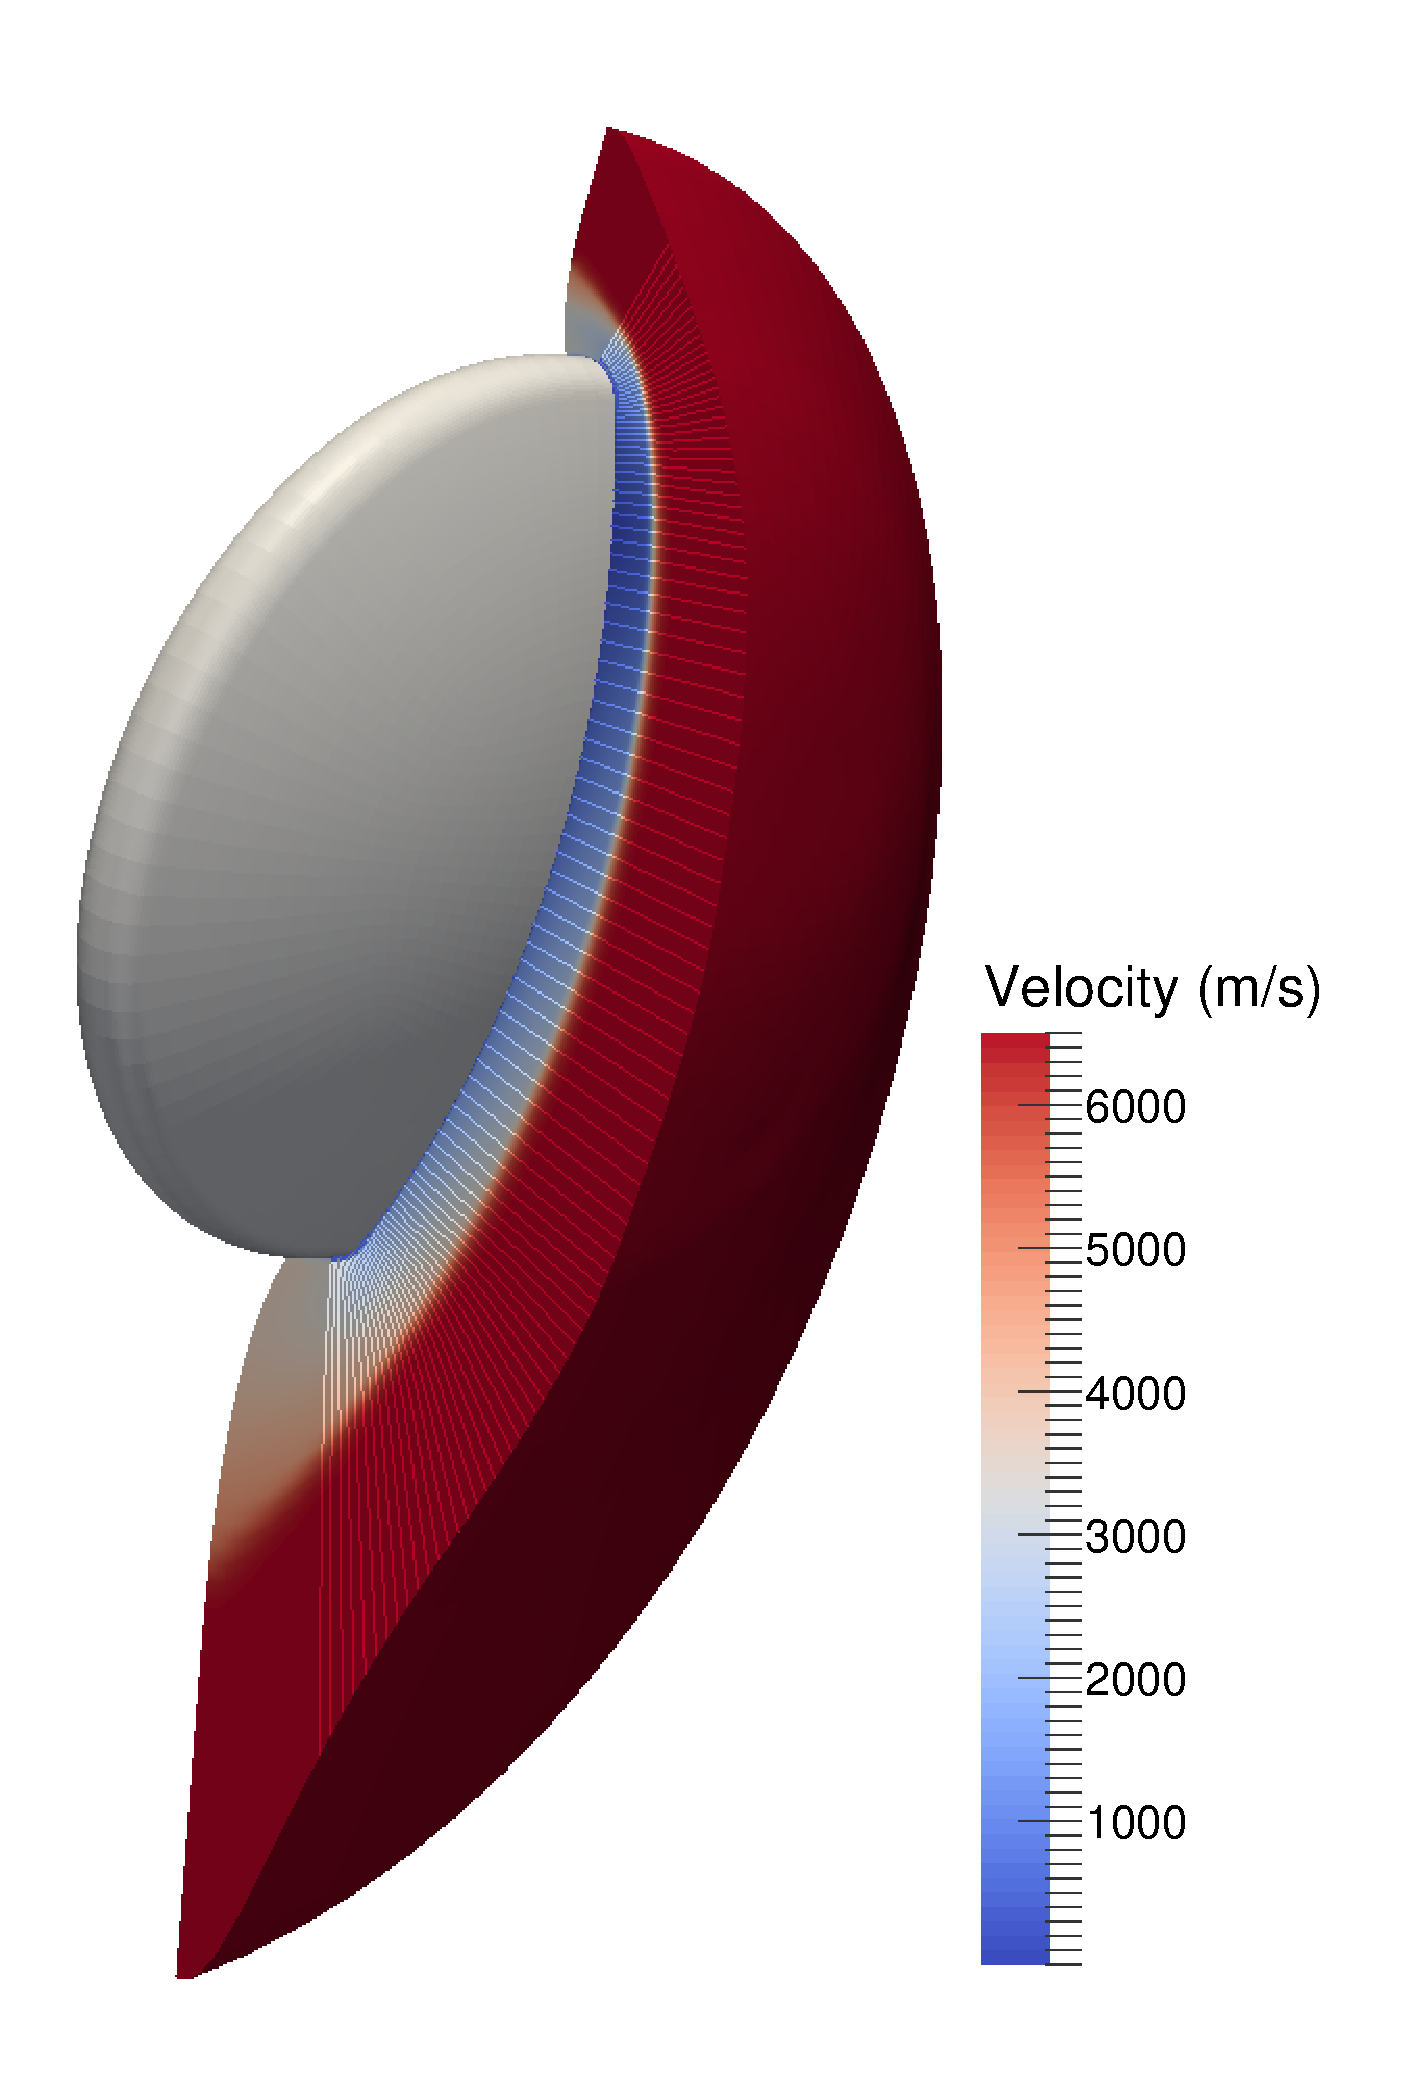
\includegraphics[height=0.50\textheight]{symplanenorm}
  \caption[
    The velocity magnitude on the symmetry plane for a fully
    laminar Orion MPCV TPS simulation
  ]{%
    \label{fig:cev_symplane}
    The velocity magnitude on the symmetry plane for a fully
    laminar Orion MPCV TPS simulation performed by P. T. Bauman.
  }
\end{figure}

%\subsection{Fully Turbulent Return from the International Space Station}

\citet{Bauman2011Loose} performed coupled multiphysics simulations of
the Orion MPCV geometry undergoing peak heating during return from
the International Space Station at a $19$\textdegree{} angle of attack.
%
A fully turbulent assumption, implemented through use of the Baldwin--Lomax
model, was applied over the entire thermal protection system (TPS) surface.
%
Local turbulent
boundary layer conditions, taken from the colored symmetry plane in
\autoref{fig:cev_symplane}, appear in \autoref{tbl:BaumanCEVConditions}.
This boundary layer data has several peculiar features.  The wall
is quite cold compared with the freestream ($T_e/T_w \approx
3.5$) causing large thermodynamic state ($\rho_e/\rho_w \approx
0.23$) and property changes ($\mu_e/\mu_w \approx 2.8$) across
the layer.  The shape factor $(\delta^\ast / \theta \approx 0.85)$
has a small value only possible in flows with significant density
variations.  The magnitude of the negative-valued Clauser parameter
$\beta$~\citep{Clauser1954Turbulent} indicates that a very strong favorable
pressure gradient is present as magnitudes like $0.1$ are considered
strong~\citep{Smith1994Effects,Luker2000Influence}.  The momentum
Reynolds numbers $\Reynolds[\theta]$ are modest with the flow
accelerating from the subsonic into the supersonic regime.
The present work cannot precisely match
these flow characteristics because aerothermochemistry is neglected.
Holding the edge Mach number constant,
\autoref{tbl:BaumanCEVConditionsPerfect} maps the data onto an ideal
air equation of state as is appropriate for the governing equations
to be presented in \autoref{sec:goveqn}.

% Culled from https://svn.ices.utexas.edu/repos/pecos/turbulence/cevBoundaryLayerData/cev1@31995
\begin{table}[p]
\centering
\caption[Reacting boundary layer conditions from
        fully turbulent Orion MPCV TPS simulations]{%
  Reacting boundary layer conditions at five representative locations within
  fully turbulent Orion MPCV TPS simulations by \citet{Bauman2011Loose}.
  Dimensional quantities use MKS units.  Data reduction by O.  Sahni and V.
  Topalian.\label{tbl:BaumanCEVConditions}
}
\renewcommand{\arraystretch}{1.3}
\begin{tabular}{l|rrrrr}
Location label & \hspace{7ex}1 & \hspace{7ex}2 & \hspace{7ex}3 & \hspace{7ex}4 & \hspace{7ex}5 \\
\hline
%$x$ position                                                                      & -4.586    & -4.483    & -4.394    & -4.325    & -4.273    \\
%$y$ position                                                                      & 0.000     & 0.000     & 0.000     & 0.000     & 0.000     \\
%$z$ position                                                                      & 1.326     & 1.719     & 1.994     & 2.182     & 2.310     \\
%$x$ edge                                                                          & -4.654    & -4.558    & -4.478    & -4.409    & -4.359    \\
%$y$ edge                                                                          & 0.000     & 0.000     & 0.000     & 0.000     & 0.000     \\
%$z$ edge                                                                          & 1.335     & 1.733     & 2.017     & 2.211     & 2.342     \\
%\hline
%$\frac{d h}{d \eta}/h \approx 0$                                                  & -1.38e-02 & -4.75e-03 & -1.21e-02 & -6.02e-03 & -8.02e-05 \\
%Max angle                                                                         & 3.8       & 4.4       & 3.3       & 2.5       & 1.8       \\
 $\delta$                                                                          & 6.95e-02  & 7.60e-02  & 8.71e-02  & 8.93e-02  & 9.19e-02  \\
 $\delta^*$                                                                        & 7.70e-03  & 8.37e-03  & 1.02e-02  & 1.02e-02  & 1.04e-02  \\
 $\theta$                                                                          & 9.49e-03  & 1.03e-02  & 1.16e-02  & 1.18e-02  & 1.20e-02  \\
 $T_w$                                                                             & 1665      & 1656      & 1646      & 1636      & 1634      \\
 $T_e$                                                                             & 5851      & 5772      & 5701      & 5647      & 5604      \\
 $\rho_w$                                                                          & 0.0148    & 0.0133    & 0.0123    & 0.0115    & 0.0109    \\
 $\rho_e$                                                                          & 0.0033    & 0.0031    & 0.0029    & 0.0027    & 0.0026    \\
 $p_e$                                                                             & 8507      & 7664      & 7066      & 6621      & 6317      \\
 $\left|\frac{d p}{d \xi}\right|_e$                                                & 2059      & 2089      & 2112      & 2171      & 2345      \\
 $\mu_w$                                                                           & 5.83e-05  & 5.81e-05  & 5.79e-05  & 5.77e-05  & 5.76e-05  \\
 $\mu_e$                                                                           & 1.64e-04  & 1.62e-04  & 1.60e-04  & 1.59e-04  & 1.58e-04  \\
 $a_e$                                                                             & 1987      & 1967      & 1949      & 1937      & 1928      \\
 $\tau_w$                                                                          & 26.72     & 29.38     & 31.13     & 32.26     & 34.89     \\
\hline
 $\Mach[e]{}$                                                                      & 0.88      & 0.99      & 1.09      & 1.15      & 1.19      \\
 $\Reynolds[\theta]{} = \frac{\rho_e u_e \theta}{\mu_e}$                           & 338       & 380       & 441       & 449       & 455       \\
 $\beta = \frac{\delta^\ast}{\tau_w}\left(\frac{\partial p}{\partial\xi}\right)_e$ & -0.59     & -0.60     & -0.69     & -0.68     & -0.70     \\
\end{tabular}
\end{table}



\begin{table}[p]
\centering
\caption[Perfect gas boundary layer conditions based on
        fully turbulent Orion MPCV TPS simulations]{%
  Translation of selected data, holding $\Mach[e]{}$ constant, from
  \autoref{tbl:BaumanCEVConditions} to $\gamma=1.4$ ideal air obeying Sutherland
  viscosity law.  Reduction by O.  Sahni and V.
  Topalian.\label{tbl:BaumanCEVConditionsPerfect}
}
\renewcommand{\arraystretch}{1.3}
\begin{tabular}{l|rrrrr}
Location label & \hspace{7ex}1 & \hspace{7ex}2 & \hspace{7ex}3 & \hspace{7ex}4 & \hspace{7ex}5 \\
\hline
 $\Mach[e]{}$                                                                      & 0.88      & 0.99      & 1.09      & 1.15      & 1.19      \\
 $\Reynolds[\theta]{} = \frac{\rho_e u_e \theta}{\mu_e}$                           & 391       & 440       & 511       & 520       & 526       \\
 $\beta = \frac{\delta^\ast}{\tau_w}\left(\frac{\partial p}{\partial\xi}\right)_e$ & -0.81     & -0.81     & -0.93     & -0.92     & -0.94     \\
\end{tabular}
\end{table}


%\subsection{Fully Laminar Return from the International Space Station}

Bauman additionally performed fully laminar simulations
of the same scenario using the {FIN-S} hypersonic flow
solver~\citep{Kirk2014Modeling}.  Post-processing along the symmetry
plane from \autoref{fig:cev_symplane} produced the reduced data depicted
in \autoref{fig:cevisslam_summary1}.  The horizontal axis measures
the distance leeward from the stagnation point taken along the MPCV's
curved heat shield.  The local surface curvature is seen to be small and
constant across a large portion of this symmetry plane.  The stagnation
condition, located at the abscissa origin, is evident in the behavior
of the momentum Reynolds number, $\Reynolds[\theta]{}$, and the edge
Mach number, $\Mach[e]$.  When measured by the outgassing velocity
normalized by viscous units, $v_w^{+}$, the ablator becomes more active as
one approaches the stagnation point.  Strong thermodynamic property variations
occur because the ablator maintains a cold surface relative to
the freestream and because of active aerothermochemistry.  The former
effect appears in the ratio of the edge-to-wall temperature,
$T_e/T_w$, and is the predominant driver between the edge-to-wall
viscosity ratio, $\mu_e/\mu_w$, causing the difference between the
two $\Reynolds[\theta]$ curves.  The lower curve, momentum Reynolds
number based on edge viscosity, is what has been discussed thus far
and what the current work predominantly uses.  Notice that absent cold
wall effects these $\Reynolds[\theta]$ are well into the range where
relaminarization is expected~\citep[\textsection{}3.2]{Spalart1988Direct}.
Temperature differences in conjunction with chemical reactions cause
wall-to-edge differences in the ratio of specific heats, $\gamma$, and in the
Prandtl number, $\Prandtl$.

\begin{figure}[p]
  \centering
  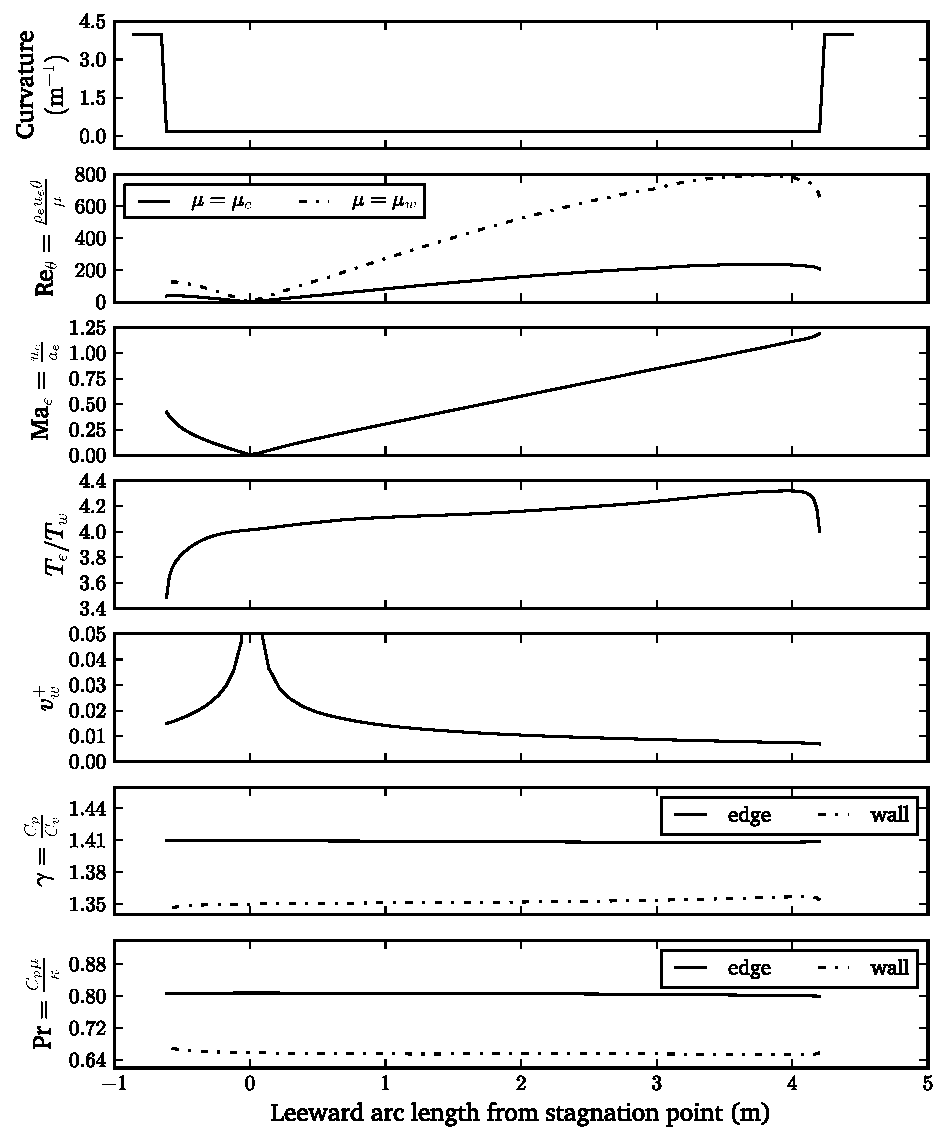
\includegraphics[height=0.95\textheight]{cevisslam_summary1}
  \caption[
    Reacting boundary layer conditions from the symmetry plane on a fully
    laminar Orion MPCV thermal protection system simulation
  ]{%
    \label{fig:cevisslam_summary1}
    Reacting boundary layer conditions from the symmetry plane on a fully
    laminar Orion MPCV TPS simulation performed by P. T. Bauman.
  }
\end{figure}

The strength of the favorable pressure gradient from this
fully laminar data has been quantified using a variety of
parameters in \autoref{fig:cevisslam_summary_fpg}.
The nondimensional quantities are the Clauser parameter
$\beta$~\citep{Clauser1954Turbulent}, Launder's acceleration parameter
$K$~\citep{Launder1964Laminarization}, the Pohlhausen parameter $K_s$~\citep{Pohlhausen1921Zur},
similarity parameter $\Lambda$~\citep{Cal2008Similarity}, parameter
$\Lambda_n$~\citep{Narasimha1979Relaminarization}, and a new
invention~$p_{e,\xi}^{\ast}$.  The figure caption shows their definitions
with $\xi$ denoting the streamwise direction and $e$ and $w$ being edge
and wall values, respectively.  Here, $\delta^\ast$ is the displacement
thickness, $\tau_w$ the wall shear stress, $\delta$ the boundary layer
thickness, and $\nu$ the kinematic viscosity.  Though physical truth would
produce smooth curves in \autoref{fig:cevisslam_summary_fpg}, numerical
artifacts are apparent despite care during the data reduction process.
They arise because the grid refinement strategies used to produce the
source data did not target these parameters.  All quantities shown become
problematic near the stagnation point.  The curves for $K_s$ and $\Lambda$
are particularly noisy due to their dependence on functions of $\delta$.

Choosing one pressure gradient parameter to match for
a turbulence-sustaining study based on this Orion MPCV data is
not entirely straightforward.  Clearly $K_s$ and $\Lambda$ are not
suitable based on their numerical issues.  $K$ shows no errant behavior
but its definition uses the streamwise velocity derivative making it
more of an acceleration parameter than a pressure gradient parameter.
%
%%The distinction does not matter in the present work but might in future
%%studies involving non-ideal equations of state.
%
Quantities $\beta$ and
$\Lambda_n$ depend on $\tau_w$ which cannot be matched \emph{a priori}
due to its dependence on turbulent behavior.  Clauser's $\beta$ is also
problematic because $\delta^\ast$ behaves atypically in the
flows of interest, as will be shown in~\autoref{sec:bldata}.

These concerns motivated defining the new parameter
\begin{align}
    \label{eq:defnpexi}
    p_{e,\xi}^\ast &= \frac{\delta}{\rho_e u_e^2}
                      \frac{\partial\!p_e}{\partial\!\xi}.
\end{align}
It nondimensionalizes the pressure gradient magnitude using freestream
kinetic energy, like $K$, but scaled using the boundary layer
thickness $\delta$ to avoid difficulties associated with $\tau_w$
and $\delta^\ast$.  \autoref{fig:cevisslam_summary_fpg} shows that this new
parameter qualitatively captures the same trends as $\beta$, $K$, and
$\Lambda_n$ while being more robust numerically.  Moreover,
in \citeauthor{Topalian2014Temporal}'s class of homogenization models
the growth rate $\operatorname{gr}_{t_0}\left(\Delta\right)$ can be
used to control $\delta$ independently of $\Reynolds[\theta]$.  Hence,
given some target thickness, one can design an inviscid base flow, as is
done in Appendix~\ref{sec:radialflow}, in order to have a homogenized direct numerical
simulation easily match $p_{e,\xi}^\ast$ \emph{a priori}.  Consequently, the present work uses
parameter~\eqref{eq:defnpexi} for scenario-matching purposes and compares it
against other measures of pressure gradient strength in
\autoref{sec:bldata}.
%
%%%EVIL%EVIL%EVIL%%%
\enlargethispage{0.25em}
%%%EVIL%EVIL%EVIL%%%

\begin{figure}[p]
  \centering
  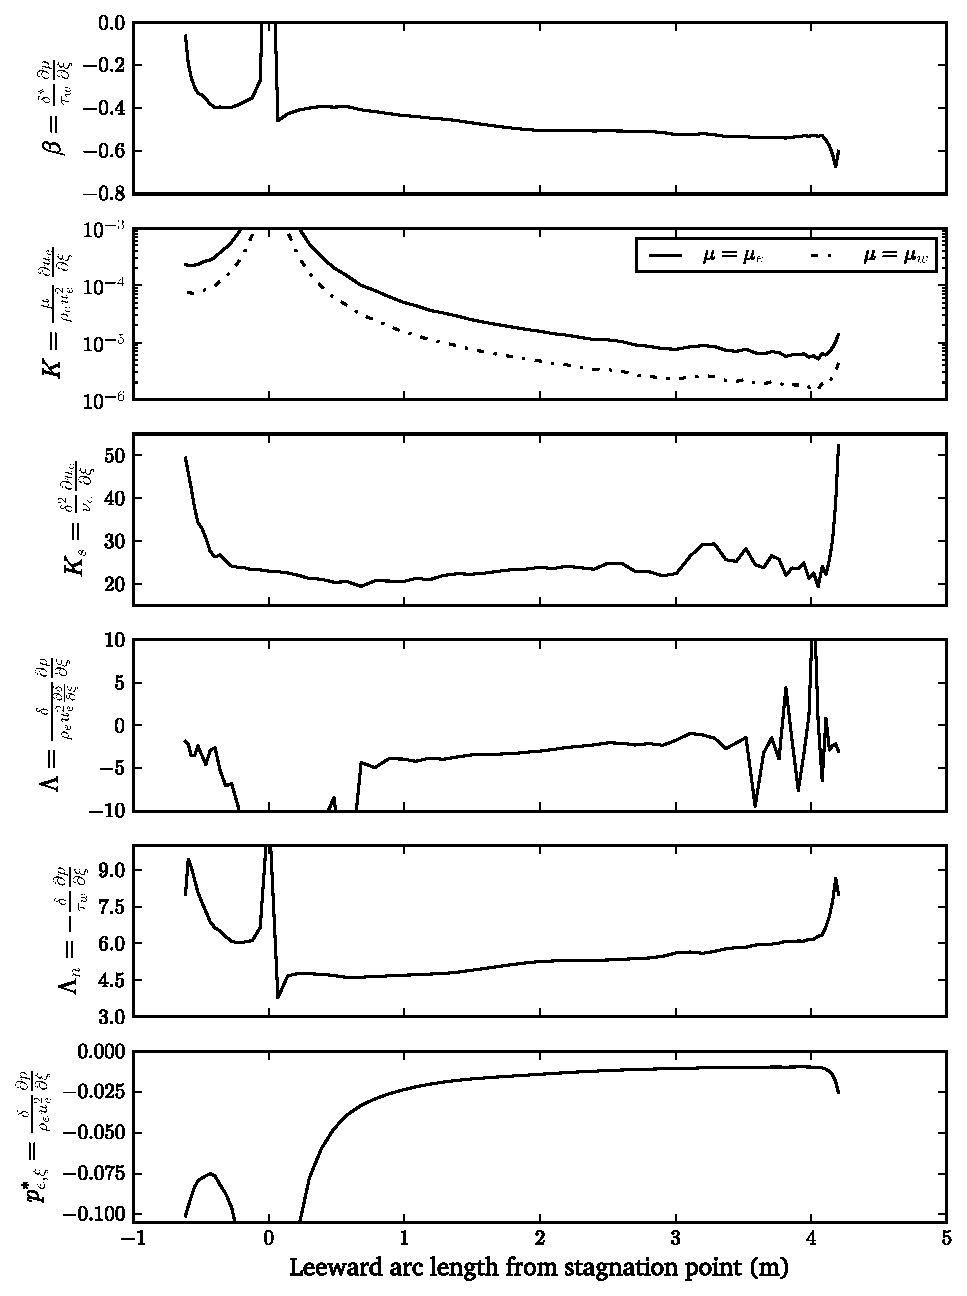
\includegraphics[height=0.95\textheight]{cevisslam_summary_fpg}
  \caption[
    Pressure gradient conditions from the symmetry plane on a fully laminar
    Orion MPCV thermal protection system simulation
  ]{%
    \label{fig:cevisslam_summary_fpg}
    Pressure gradient conditions from the symmetry plane on a fully laminar
    Orion MPCV TPS simulation performed by P. T. Bauman.
  }
\end{figure}

\clearpage
